\documentclass[11pt,a4paper]{report}		                                   

\usepackage{graphicx}
\usepackage{a4}
\usepackage{german}
\usepackage[utf8]{inputenc}
\usepackage{listings}
\usepackage{cite}
%\usepackage[square, numbers]{natbib}
\usepackage{here}
\usepackage[hidelinks, urlcolor=blue]{hyperref}
%\usepackage{xr}
\usepackage[numbers]{natbib}

\newcommand{\Mycite}[1]{%
	\citeauthor{#1}~\citeyear{#1}}
\newcommand{\Myciten}[2]{%
	\citeauthor{#1}~\citeyear{#1}, S.#2}
%\setcitestyle{authoryear,open={},close={}, notesep={:}}



\usepackage{color}
\usepackage{textcomp}

\definecolor{listinggray}{gray}{0.9}
\definecolor{lbcolor}{rgb}{0.9,0.9,0.9}
\definecolor{stringcolor}{RGB}{32,108,32}

\lstdefinestyle{scala}{
	morekeywords={ abstract,case,catch,
    char,class,
    def,else,extends,final,
    if,import,
    match,module,new,null,object,
    override,package,private,protected,
    public,return,super,this,throw,
    trait,try,type,val,var,with,implicit,
    macro,sealed
  },
 	morestring=[b]",
	morestring=[b]""",
	%backgroundcolor=\color{lbcolor},
	%tabsize=4,
	%rulecolor=,
	%language=scala,
    %basicstyle=\scriptsize,
    %upquote=true,
    aboveskip={1.5\baselineskip},
    %columns=fixed,
    %showstringspaces=false,
    extendedchars=true,
    breaklines=true, %sorgt dafür, dass Text, der die Formattierung sprengt in die nächste Zeile rückt
    %prebreak = \raisebox{0ex}[0ex][0ex]{\ensuremath{\hookleftarrow}}, %sorgt dafür, dass eingerückte Zeilen über ein 'return' zeichen angekündigt werden
    frame=single, % sorgt dafür dass ein Rand eingezeichnet wird
    showtabs=false,
    captionpos=b,
    showspaces=false,
    showstringspaces=false,
    identifierstyle=\ttfamily,
    keywordstyle=\color[rgb]{0,0,1},
    commentstyle=\color[rgb]{0.133,0.545,0.133},
    stringstyle=\color{stringcolor},
    literate=%
  {Ö}{{\"O}}1
  {Ä}{{\"A}}1
  {Ü}{{\"U}}1
  {ß}{{\ss}}2
  {ü}{{\"u}}1
  {ä}{{\"a}}1
  {ö}{{\"o}}1
  {~} {$\sim$}{1}
}

\lstdefinestyle{spray}{
	morekeywords={style, shape, diagram, connection, for, extends, ellipse, rectangle, roundedrectangle, polygon, polyline, text, description},
	morestring=[b]",
	morestring=[b]""",
	%backgroundcolor=\color{lbcolor},
    aboveskip={1.5\baselineskip},
    extendedchars=true,
    breaklines=true, %sorgt dafür, dass Text, der die Formattierung sprengt in die nächste Zeile rückt
    showtabs=false,
    captionpos=b,
    frame=single,
    showspaces=false,
    showstringspaces=false,
    identifierstyle=\ttfamily,
    keywordstyle=\color[rgb]{0,0,1},
    commentstyle=\color[rgb]{0.133,0.545,0.133},
    stringstyle=\color{stringcolor},
    literate=%
  {Ö}{{\"O}}1
  {Ä}{{\"A}}1
  {Ü}{{\"U}}1
  {ß}{{\ss}}2
  {ü}{{\"u}}1
  {ä}{{\"a}}1
  {ö}{{\"o}}1
  {~} {$\sim$}{1}
}


\newcommand{\thema}{Scala als Generatorensprache zur Erzeugung graphischer Editoren / Eine Studie auf Umsetzbarkeit }
\newcommand{\schlagworte}{Scala, MoDiGen, Model-Driven Software Development (MDSD), Domain-Specific Language (DSL), Parser, Generatoren}
\newcommand{\zusammenfassung}{Das MoDiGen Projekt will das Erzeugen graphischer Editoren schnell und unkompliziert ermöglichen. Hierfür werden nach einem Set textueller DSLs Modellklassen erzeugt, welche die graphischen Elemente abbilden. Bisher wurde Xtext benutzt um die dafür nötigen Objektstrukturen, Parser und Generatoren erzeugen zu lassen. Da Das Projekt langsam kontinuierlich auf Scala als Programmiersprache umsteigt, soll nun untersucht werden, ob die gegebenen Funktionalitäten von Xtext in Scala umgesetzt werden können und ob Features implementiert werden können, die Xtext nicht bietet. Es werden also die gewünschten Objektstrukturen der Modellklassen umgesetzt. Außerdem werden die nötigen Parser und Generatorenklassen erstellt. Dabei spielen Vorgaben wie Vererbung und die transitive Weitergabe der Objekteigenschaften eine wichtige Rolle.}
\newcommand{\ausgabedatum}{15.11.2015}
\newcommand{\abgabedatum}{15.02.2016}
\newcommand{\autor}{Julian Müller}
\newcommand{\autorStrasse}{Mondrauteweg}
\newcommand{\autorPLZ}{78467}
\newcommand{\autorOrt}{Konstanz}
\newcommand{\autorGeburtsort}{Donaueschingen}
\newcommand{\autorGeburtsdatum}{07.07.1991 }
\newcommand{\prueferA}{Prof. Doc. Marko Boger}
\newcommand{\prueferB}{Titel, Markus Gerhart}
\newcommand{\firma}{HTWG Konstanz}
\newcommand{\studiengang}{Angewandte Informatik/Softwareengineering}



\begin{document}
\pagenumbering{gobble}

\begin{titlepage}

\vspace*{-3.5cm}

\begin{flushleft}
\hspace*{-1cm} 
\includegraphics[width=15.7cm]{htwg-logo}
\end{flushleft}

\vspace{2.5cm}

\begin{center}
	\huge{
		\textbf{\thema} \\[5cm]
	}
	\Large{
		\textbf{\autor}} \\[6.5cm]
	\large{
		\textbf{Konstanz, \abgabedatum} \\[2.3cm]
	}
	
	\Huge{
		\textbf{{\sf BACHELORARBEIT}}
	}
\end{center}

\end{titlepage}

\thispagestyle{empty}
{
\setlength{\parskip}{0.5cm}
        \begin{center}
        \textbf{\huge BACHELORARBEIT}

        \textbf{zur Erlangung des akademischen Grades}

        \textbf{\Large Bachelor of Science (B. Sc.)}

        \textbf{an der}

        \textsf{\huge Hochschule Konstanz}\\
        {\small Technik, Wirtschaft und Gestaltung}

        \textsf{\Large Fakult"at Informatik} \\
        Studiengang \studiengang
        \end{center}
}
\begin{center}

\vspace*{2cm}

\begin{tabular}{p{3cm}p{10cm}}
Thema: & \textbf{\large \thema} \\[15ex]
Bachelorkandidat: & \autor, \autorStrasse, \autorPLZ  \autorOrt \\[15ex]
1. Pr"ufer: & \prueferA \\
2. Pr"ufer: & \prueferB \\[25ex]
Ausgabedatum: & \ausgabedatum \\
Abgabedatum: & \abgabedatum \\
\end{tabular}
\end{center}

\begin{center}
{\Large \textbf{Zusammenfassung (Abstract)}}
\end{center}

\bigskip

\begin{center}
	\begin{tabular}{p{2.8cm}p{10cm}}
		Thema: & \thema \\
		 & \\
		Bachelorkandidat: & \autor \\
		 & \\
		Firma: & \firma \\
		 & \\
		Betreuer: & \prueferA  \\[.5ex]
		 &  \prueferB \\
		 & \\
		Abgabedatum: & \abgabedatum \\
		 & \\
		Schlagworte: & \schlagworte \\
		 & \\
	\end{tabular}
\end{center}

\bigskip

\noindent
\zusammenfassung
\pagenumbering{Roman}
\chapter*{Ehrenw"ortliche Erkl"arung}
\addcontentsline{toc}{chapter}{Ehrenw"ortliche Erkl"arung}

Hiermit erkl"are ich
\textit{\autor, geboren am \autorGeburtsdatum in \autorGeburtsort}, dass ich\\

\begin{tabular}{lp{12cm}}
(1) & meine Bachelorarbeit mit dem Titel \\[1em]
& \textbf{\thema} \\[1em]
& bei der \firma\ unter Anleitung von \prueferA\ selbst"andig und ohne fremde Hilfe angefertigt und keine anderen als die angef"uhrten Hilfen benutzt habe;\\[1em]
(2) & die "Ubernahme w"ortlicher Zitate, von Tabellen, Zeichnungen, Bildern und
Programmen aus der Literatur oder anderen Quellen (Internet) sowie die Verwendung
der Gedanken anderer Autoren an den entsprechenden Stellen innerhalb der Arbeit
gekennzeichnet habe.\\
\end{tabular}

\vspace*{1cm}

\noindent
Ich bin mir bewusst, dass eine falsche Erkl"arung rechtliche Folgen haben wird.\\

\vspace*{3cm}

\noindent
Konstanz, \abgabedatum \hfill \begin{tabular}{c} \\ \\ \rule{5cm}{1pt} \\ (Unterschrift)\end{tabular}

\addcontentsline{toc}{chapter}{\listfigurename}
\listoffigures
\addcontentsline{toc}{chapter}{Listings}
\lstlistoflistings
\tableofcontents
\newpage
\pagenumbering{arabic}
\setcounter{page}{1}
\chapter{Einleitung}
Seitdem Rechner mit Maschinencode programmiert werden, steigt das Abstraktionslevel der Programmiersprachen kontinuierlich an (siehe Abbildung \ref{paradigmnsintime}). Wer die Assemblersprachen kennt und fürchtet, weiß Programmiersprachen wie Fortran, Pascal oder C zu schätzen, da sie Kontrollstrukturen einführen, welche leicht verstanden und eingesetzt werden können. Wer stets wiederkehrende Muster programmiert, bedient sich der Objektorientierten Sprachen, wie zum Beispiel Java oder C++.
Indem die Logik hinter Programmiersprachen den Paradigmen angeglichen werden, die die Menschen intuitiv(oder am einfachsten) beherrschen, wird Programmieren erheblich effizienter, sowohl im Lernprozess, als auch in der Umsetzung. 
Der prozentuale Anteil an wiederverwendbarem Code in einem Projekt steigt mit dem Abstraktionslevel der verwendeten Programmierparadigmen. Code, der wiederverwendet werden kann, spart Zeit und reduziert die Chance neue Fehler in das Projekt einzuarbeiten. Die Objektorientierung wurde eingeführt um wiederkehrende Elemente einheitlich behandeln zu können (z.B. graphische Elemente), somit die Komplexität des Codes zu verringern und dessen Wartbarkeit zu erleichtern. Die Programmiersprache \textit{Scala} ist ebenfalls objektorientiert, erfüllt jedoch ebenso die Kriterien einer funktionalen Programmiersprache und bietet zudem einige Features, die sie besonders dafür qualifizieren, sogenannte \textit{Domain Specific Languages} zu erstellen. Dies begünstigt die Unterstützung des nächsten Schrittes in der Evolution der Programmierparadigmen. Nicht zuletzt der Markt bekräftigt den Wunsch nach eben dieser Effizienz und fordert diese nächste Abstraktionsstufe. 
\begin{figure}[h]
	\begin{center}
		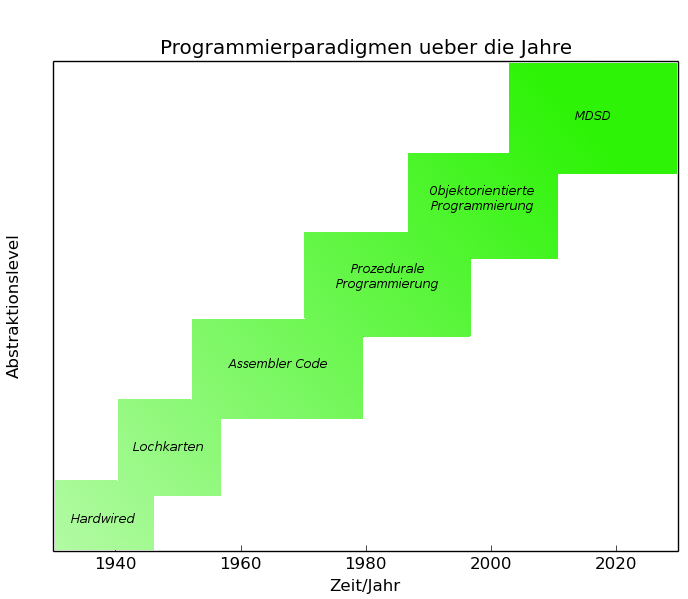
\includegraphics[width = \textwidth]{Bilder/paradigmsInTime(matplotlib).png}
		\caption{Programmierparadigmen im Verlauf der Zeit}
		\label{paradigmnsintime}
	\end{center}
\end{figure}Entwickler auf der ganzen Welt benutzen Bibliotheken und Frameworks, um bereits entwickelte Lösungen wiederverwenden zu können und um bekannte Lösungsansätze für bekannte Problemstellungen zu verwenden. Der hierbei entwickelte Code richtet sich also nach einem bereits vorgelegten Plan. Jener Quellcode, der manuell ergänzt werden muss, lässt sich nun teilweise automatisiert ergänzen.  Dieses Ziel verfolgt das \textbf{M}odel \textbf{D}riven \textbf{S}oftware \textbf{D}evelopment (\textit{MDSD}). Schematischer Code kann in domänenspezifischen Modellen verarbeitet werden. Nachdem Modelle konzipiert sind, ist es möglich automatisiert auf domänenspezifische Problemstellungen einzugehen. Im Falle der Industrie bedeutet dies Massenproduktion, ermöglicht von Robotern. In Bezug auf Softwareentwicklung, bedeutet dies Code, der Code generiert. Die Idee ist, variable Teile des Codes über ein Modell zu beschreiben. Das Programm ist selbstständig in der Lage, das Modell in den gewünschten Code umzuwandeln. Das besagte Modell kann hierbei drastisch vereinfacht, oder auf eine bestimmte Benutzerzielgruppe(Domäne) angepasst sein. Es lässt sich also problemlos einrichten, beispielsweise einem Banker über seine gewohnten Fachbegriffe eine \textbf{D}omain \textbf{S}pecific \textbf{L}anguage (\textit{DSL}) zu bieten, welche syntaktisch auch noch einer seiner Tabellen oder beispielsweise Buchungssätzen ähnelt und somit für ihn unkompliziert und sofort erlernbar ist. Für die Umwandlung eines Modells in konkreten Code (Generat) sind sogenannte Generatoren notwendig. 
\linebreak 
Siehe auch \Mycite{trompeter:mda}

\section{Was Ist MoDiGen?}\label{modigen}
Domänenspezifische Modellierung erfreut sich wachsender Beliebtheit in der Softwareentwicklung. Projekte, die für ein domänenspezifisches Problem graphische Modellierungstools benötigen, können entweder ein sehr spezifisches Tool benutzen, was nur dann möglich ist, wenn das Problem exakt durch das Tool beschrieben werden kann. Ansonsten muss ein generischer Editor herangezogen werden, doch diese sind dann in der Regel derart komplex, dass es nicht mehr möglich ist, sein Problem schnell und unkompliziert darstellen zu können. Das \textit{MoDiGen} (\textbf{Mo}del \textbf{Di}agram \textbf{Gen}erator) Projekt will es ermöglichen, durch kurze und schnell umsetzbare textuelle DSLs, graphische Editoren erzeugen zu lassen, deren Entwicklung sonst überaus zeitaufwendig sein kann. Hierfür wurde einerseits ein hoch abstrahiertes Metamodell erstellt, das komplexe Klassenhierarchien darstellen kann, außerdem wurden einige textuelle DSLs erstellt, über die die Modellklassen beschrieben werden können (Diagram, Shape, Connection, Style). So soll dem Anwender (\textit{Domain Expert}) die Möglichkeit geboten werden, eigene graphische Elemente zu erzeugen. Dabei kann es sich auch um Verbindungselemente handeln, denn diese werden im Metamodell von MoDiGen getrennt und ebenbürtig zu den eigentlichen Elementen gehandhabt (vgl. \Mycite{gerhart:modigen_concept}). Außerdem werden sie nicht wie bei etwa \textit{Ecore} nur als Attribut eines Modells gehalten. Im Hinblick auf die Skalierbarkeit ist dies vorteilhaft, da Elemente nicht über ein relationales Schema abgebildet werden müssen, um sie in einer Datenbank zu hinterlegen. Hieraus entstehen wiederum Vorteile bezüglich der Skalierbarkeit und des Datenzugriffs.
\section{Aufgabenstellung}
Hinsichtlich der Flexibilität der Modelle und der Skalierbarkeit, bieten bestehende Lösungen wie \textit{Xtext} und \textit{Ecore} derzeit keine Ideale Lösung. Die relativ junge Programmiersprache \textit{Scala} ist, wie der Name schon andeuten soll, mit einem besonderen Fokus auf die Skalierbarkeit entwickelt worden. Wie bereits in \ref{modigen} erläutert, stützt sich das MoDiGen Projekt auf ein neues, selbst entwickeltes Metamodell, welches hinsichtlich der Skalierbarkeit und der Speicherauslastung wesentlich bessere Ergebnisse erzielt. So wie das Metamodell sollen nun auch die Parser und Generatoren in Scala umgesetzt werden. Es soll untersucht werden, inwiefern Scala (als allzweckstaugliche Programmiersprache) sich dafür eignet, die Rolle bestehender spezialisierter Technologien zu übernehmen. Wo kann Scala seine Stärken spielen lassen und wo ist es den bisherigen Lösungen unterlegen? Dafür sollen u.a. MoDiGens Modellklassen: Style, Shape und Diagram in Scala umgesetzt werden und die entsprechenden Parser und Generatoren erstellt werden. Konkreter: Es müssen zunächst die geforderten Objektstrukturen geschaffen werden um Style, Shape und Diagram abbilden zu können. Hierbei muss darauf geachtet werden, dass ein Style ein weiteres Style assoziieren kann um eine Vererbung zu ermöglichen.\\\\Shapes können derzeit aufgrund der Komplexität der Modellklasse nicht vererbt werden. Sowohl die Shapevererbung als auch Mehrfachvererbung im allgemeinen ist mit bestehenden Technologien nicht möglich und soll daher auf Umsetzbarkeit mit Scala überprüft werden. Des weiteren sind die Beziehungen der Modelle untereinander genau geklärt - siehe Abbildung \ref{diagramshapestyle}. Diagrams können auf Styles und Shapes verweisen und Shapes können Styles referenzieren.\\\\Außerdem muss ein Parser erstellt werden, der in der Lage ist die \textit{Spray} DSL zu interpretieren und entsprechend der Modelle zu instantiieren. Zuletzt kommen Generatorenklassen, die schließlich entsprechende Generate aus den erzeugten Objekten erstellen können. Es handelt sich also um eine Studie zur Umsetzbarkeit von Parser- und Generatorenklassen in Scala, mit speziellem Fokus auf die Möglichkeit komplexe Vererbungshierarchien darstellen zu können. Hierbei liegt die größte Herausforderung darin, einen Parsingmechanismus zu erstellen, der mit rekursiven DSL Definitionen umgehen kann und der unabhängig davon um welche Modellklasse es sich handelt, in der Lage ist Vererbungshierarchien zu erkennen und umzusetzen. Da der Autor Scala erst für dieses Projekt erlernt, kann davon ausgegangen werden, dass alle verwendeten Techniken anfängerfreundlich sind.
\begin{figure}[h]
\begin{center}
\includegraphics[scale = 0.7]{Bilder/vereinfachteobjektstruktur.png}
%\includegraphics[width = \textwidth]{Bilder/vereinfachteobjektstruktur.png}
\caption{Klassendiagramm Diagram, Shape, Style (Sehr stark vereinfacht)}
\label{diagramshapestyle}
\end{center}
\end{figure}
\chapter{Grundlagen: Scala/Xtext}
\section{Scala}
Im folgenden soll zum Verständnis zunächst die Programmiersprache Scala vorgestellt werden.
Die Entwicklung von Scala (Scalable Language) begann bereits 2001 an der École polytechnique fédérale de Lausanne in der Schweiz von einem Team um Professor Martin Odersky. Designziel war eine elegante, typsichere Programmierung, vollkommene Kompatibilität mit der JVM und eine Zusammenführung der Objektorientierung und der funktionalen Programmierung (vgl. \cite{braun:scala}). Scala ist hierbei objektorientierter als z.B. Java, da in Scala \textit{alles} ein Objekt ist. Odersky selber bezeichnet Scala als postfunktionale Sprache, da immernoch diskutiert wird, ob Scala als funktionale Programmiersprache betitelt werden darf. Fest steht jedoch, dass man in Scala funktional programmieren kann - man muss es allerdings nicht. Funktionen können Argumente oder Ergebnisse anderer Funktionen sein und sind somit \textit{Higher Order Functions}. Trotz der Typsicherheit bietet Scala das \textit{Feeling} einer dynamisch typisierten Sprache, da Typen beim Überetzen inferiert werden können. Der Compiler erkennt also anhand des initialisierten Wertes, um was für einen Typ es sich handelt, so kann fast immer auf manuelle Typkennzeichnung verzichtet werden.
\begin{lstlisting}[style = scala]
val name = "Julian"
val alter = 24
\end{lstlisting}
sind vollkommen korrekte Ausdrücke und werden ebenso kompiliert wie:
\begin{lstlisting}[style = scala]
val name:String = "Frederik"
val alter:Int = 33
\end{lstlisting}
Scala ist einfacher zu erlernen, als beispielsweise Java, da Anweisungen auch alleinstehend als Skript oder direkt in einem interaktiven Scalainterpreter ausgeführt und ausprobiert werden können. 
Komplexe Problemstellungen können stark abstrahiert in wenigen Zeilen Code beschrieben werden. Über entsprechende Methoden, kann man sogar eigene Operatoren und Kontrollstrukturen erstellen \textit{"`Damit ist Scala prädestiniert zur Erstellung von Domain Specific Languages $[$...$]$"'.} \citet[p. 2]{braun:scala}
%TODO Beispiel
\section{Xtext}\label{xtext}
Nachdem nun Scala erörtert wurde, soll im folgenden die zu ersetzende Technologie \textit{Xtext} erklärt werden.
\textit{"`Xtext ist ein Framework zum Erstellen von Programmiersprachen und \textbf{D}omain-\textbf{S}pecific \textbf{L}anguages. Mit Xtext wird deine Programmiersprache durch eine mächtige Gramatiksprache definiert"'} $\sim$ \citet{xtext:website}.
Xtext ist ein Framework mit dem u.a. Domänenspezifische Sprachen entwickelt werden können und ergänzt das \textit{Eclipse-Modeling-Framework}\cite{emf}. Dafür wird eine komplexe Grammatiksprache zur Vergügung gestellt, über die Entitäten deklariert und assoziiert werden können. Anhand der Grammatik erzeugt Xtext Parser, Generatoren und sogar ein Klassenmodell für die beschriebenen Klassen (vgl. \citet{xtext:goodbyexml}). Um die beschriebene \textit{DSL} ausführbar zu machen wird außerdem ein Texteditor generiert, welcher entsprechendes Syntax Highlighting automatisch programmiert. Der große Vorteil von Xtext ist, dass die Definition der beschriebenen Sprache gleichzeitig die Objektstruktur der zu generierenden Modelle beschreibt. Wird die Objektstruktur der Modelle verändert, ändert sich die DSL ebenfalls und so bleibt die Abbildung von DSL auf Modell immer konsistent. 
%TODO: Hinführung,in welchen Bereichen wird Xtex eingesetzt, Beispiel, Positives/Negatives

\chapter{Ansatz}\label{ansatz}
Nachdem die Problemstellung geklärt ist und die konkurrierenden Technologien erläutert wurden, sollen nun die zugrundeliegenden Gedanken zur Problemlösung vorgestellt werden. Die hier aufgeführten Konzepte für Beispiele verwendete Methoden- oder Klassennamen entsprechen nicht zwingend der tatsächlichen Umsetzung.
\section{Objektstruktur}
Zunächst werden die entsprechenden Modellklassen aus der Xtext Grammatik in Scala Quellcode übernommen. Style-, Shape-, Connection- und Diagram Klassen mit entsprechenden Feldern werden zunächst als sogenannte \textit{case classes} erstellt. Dies hat den Vorteil, dass im Falle einer später notwendigen Verifizierung der Instanzen, vorimplementierte \textit{hash}- \textit{equals}- und \textit{toString} Methoden zur Verfügung zu haben. Da Style am flexibelsten ist (nur eingehende Abhängigkeiten), wird Style.scala zuerst erstellt und entsprechend der Assoziationsreihenfolge dann Shape.scala und Diagram.scala (siehe Abbildung \ref{diagramshapestyle}).
\subsection{ClassHierarchy}Da es für die Instanzen mancher Modellklassen möglich sein soll, Objekte der selben Klasse zu erweitern, ist die Idee des Autors, eine Collection namens \textit{ClassHierarchy} zu erstellen, welche in der Lage ist, ähnlich eines Baumes Vererbungshierarchien in Form von Knoten (\textit{Nodes}) darzustellen. Siehe dazu Abbildung \ref{classhierarchy}. So werden die Modellklassen, für die die Vererbung möglich sein soll, über diesen Baum in Relation gesetzt. Im Falle einer gänzlich neuen Modellklasse (z.B. ein neuer Style), wird die Instanz als neue Basisklasse eingefügt. Ansonsten über eine Methode, die beispielsweise \textit{inheritsFrom} heißen könnte. \textit{InheritsFrom} muss entweder von der \textit{ClassHierarchy} oder den Knoten selber zur Verfügung gestellt werden. Über die entsprechende Argumentenliste wird vermittelt, welche Knoten erweitert werden. \textit{InheritsFrom} ergänzt dann eigenständig die \textit{parent}- und \textit{children} Listen eines Knotens um die neue Instanz der Modellklasse.
\begin{figure}[H]
\begin{center}
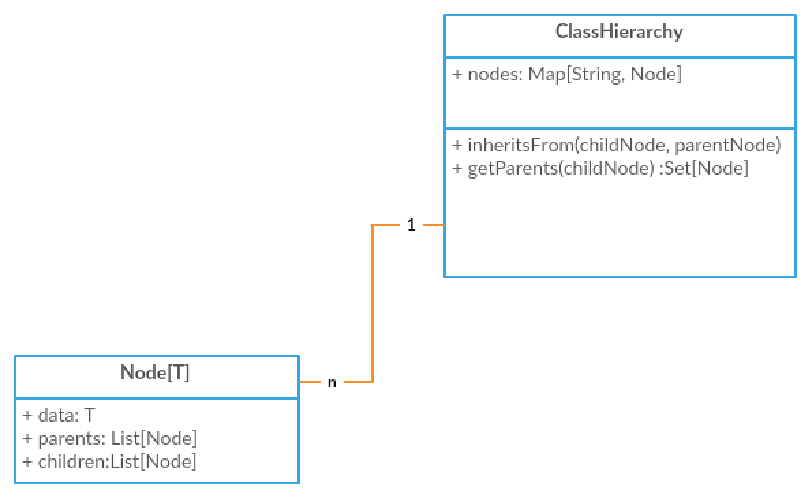
\includegraphics[scale = 0.7]{Bilder/classhierarchy.pdf}
\caption{Klassenmodell von ClassHierarchy}
\label{classhierarchy}
\end{center}
\end{figure}Wie in \ref{classhierarchy} zu sehen ist verfügen die Nodes über Listen, welche auf Eltern- und auf Kind knoten verweisen. So kann man bequem von jedem Style erfahren, welche Styles er erweitert und welche Styles ihn erweitern. Außerdem enthält \textit{ClassHierarchy} eine Map, die Namen (Strings) auf beliebige Klassen abbilden kann. Über dieses mapping ist ein schneller Zugriff auf die gewünschte Klasse möglich, ohne mühsam durch eine Baumstruktur der Nodes navigieren zu müssen.
Um dieses Prinzip auf alle möglichen Klassen anwenden zu können, sollte \textit{ClassHierarchy} generisch sein. Vorausgehend waren die Anforderungen für Vererbung nur auf Style bezogen. Da die Vererbungsprinzipien aber auch bei Shape hilfreich sein könnten, ist so gewährleistet, dass man sich diese Tür nicht unnötig verschließt. 
Benötigte Enumerationen und andere nicht komplexe Hilfsobjekte der Klassen werden in dessen \textit{Companion Objekt} definiert. 
Über entsprechende \textit{Apply}-Methoden wird der Aufruf der \textit{ClassHierarchy} so einfach wie möglich gestaltet (siehe Listing \ref{lst:applyadvance}, Zeile 2).
\begin{lstlisting}[style=scala, caption = {Beispielhafte Vereinfachung durch Apply Methode}, label = {lst:applyadvance}]
classHierarchy.nodes.get("styleName").data
classHierarchy("styleName")
\end{lstlisting}Zeile 1 in Listing \ref{lst:applyadvance} zeigt wie der Aufruf eigentlich ausshen müsste. Zeile 2 hingegen ist kürzer und außerdem verständlicher.
Da der Aufruf in diesem Fall sehr eindeutig ist, kann ruhigen Gewissens auf die Apply-Methode zurückgegriffen werden. "`\textit{Fazit: Die Methoden apply und update sollten nur eingesetzt werden, wenn intuitiv klar ist was der Einsatz der Klammern bedeutet}"'(\Myciten{esser:scala}{76}).

\section{Parser}Neben den Gedanken zur Vererbung der Modellklassen, ist es auch wichtig zu klären, wie die Modelle überhaupt aus der Stringform in Objektform umzuwandeln sind. Entsprechende Mechanismen werden allgemein als Parser bezeichnet. Dieser Parser ist verantwortlich dafür die in Stringform enthaltenen Styles, Shapes, Connections und Diagrams als diese zu identifizieren und in Objekte umzuwandeln. 
Die Struktur eines Styles (ähnlich auch bei den anderen Modellen) ist in Listing \ref{lst:beispielstyle} beispielhaft dargestellt.
\begin{center}
\label{lst:beispielstyle}
\begin{lstlisting}[style=spray, caption={Beispielhafte Style Definition über die entsprechende Style DSL},label={lst:beispielstyle}]
style BpmnDefaultStyle {

	description = "The default style of the petrinet diagram type."
	
	transparency = 0.95

	background-color = black
	
	line-color = black

	line-width = 1

	font-color = black

	font-name = "Tahoma"
	
	font-size = 6

	font-bold = yes

	font-italic = yeshttp://www.macwrench.de/wiki/Kurztipp_-_Quellcodelistings_in_LaTeX

	gradient-orientation = horizontal
	und
}
\end{lstlisting}
\end{center}
Die Xtext Grammatik soll außerdem um eine Vererbungskomponente erweitert werden, die einerseits auch Shapes die Möglichkeit bietet andere Shapes zu erweitern. Zusätzlich soll auch Mehrfachvererbung untersucht und gegebenenfalls umgesetzt werden. Shapes sollen also so definiert werden können wie in Listing \ref{lst:shapeextends} zu sehen ist.
\begin{lstlisting}[style=spray, caption = {(Mehrfach)Vererbung bei einer Shape Definition}, label = {lst:shapeextends}]
shape SomeShape extends StandardShape, AnotherShape {...}
\end{lstlisting}Es ist zwar bereits möglich, Style zu erweitern, doch was die Vererbung von Shapes und Mehrfachvererbung generell angeht besteht noch Bedarf, da Xtext nicht in der Lage ist, diese Features umzusetzen.
\subsection{Parsing Mechanismus und Parserlogik}\label{ansatzlexer}Im Folgenden wird eine konkrete Technik vorgestellt, mit der das Umwandeln von Strings in Objekte erfolgen kann,
die sogenannten \textit{Regulären Ausdrücke}. Über diese regulären Ausdrücke kann der Style gefiltert werden, um so an der Syntax der DSL vorbei zu kommen und an die eigentlichen Attribute zu gelangen.
Anhand des ersten Wortes, soll der Parser erkennen, um welchen Modelltyp (Style, Shape, Diagram) es sich handelt. 
Weiter würde ein vordefiniertes Schlüsselwort \textit{extends} eine zu erweiternde Instanz kennzeichnen. Im Gegensatz zu diesen hart kodierten Schlüsselwörtern, werden eigentliche Attribute wie zum Beispiel \textit{line-width} zunächst unter einheitlichen Regeln geparst
und erst in einer tieferen Parser klasse oder dem entsprechenden Konstruktor aufgelöst. Auf diese Art und Weise reichen wenige Regeln aus, um komplexe Ausdrücke abbilden zu können. So geparste Attribute bleiben zunächst in der Stringform. Ziel dieses Vorgehens ist es zunächst nur Attributsname und Attributswert zu ermitteln, sicherzustellen, dass Syntaxregeln eingehalten wurden und die Weitergabe eines einheitlichen Datentyps an tiefer liegende Parserklassen. Diese erste Schicht des Parsers wird also noch keine Objekte, oder gar Baumstrukturen erzeugen, sondern lediglich alle Informationen aus dem String extrahieren, die an einen spezifischen und spezialisierten Parser weiter gegeben werden kann.
Logisch wird hierdurch das Prinzip sogenannter \textit{Lexer} dargestellt, welche insbesondere bei \textit{Compilern} Anwendung finden (vgl. \Myciten{parsing}{135}). Im Prinzip wird aber nichts anderes gemacht als eine vordefinierte Sprache zu lesen und umzusetzen, weshalb das Prinzip des Lexers auch hier sinnvoll ist.
Die vordefinierte DSL kann so auch im Bezug auf die Modellklassen leichter modifiziert werden, da solang die Syntaxregeln der DSL nicht geändert werden, der Lexer von neuen Attributen unbeeindruckt ist. Erst die spezifischen Parser müssten bei einer Solchen Änderung um eine Regel erweitert werden, welche in der Lage ist die eigentliche Information aus dem neuen Argument zu extrahieren.
Die wenig komplexen Styles sollten so einfach zu parsen sein. Shapes stellen den schwierigsten Teil beim Parsen dar, da geometrische Figuren(\textit{GeometricModel}), wie Ellipsen oder Polygone ineinander geschachtelt werden können.
\subsection{Factory Klassen}
Es wird davon ausgegangen, dass Modellklassen durch Umwandlung aus einem bereitgestellten Stringinput erzeugt werden. Dieser Stringinput enthält alle notwendigen Informationen um eine einsatzfähige Instanz einer Modellklasse erzeugen zu können. Es ist wünschenswert die Erzeugung der Instanzen so konsistent wie möglich zu halten. Dies bedeutet möglichst wenige und klar definierte Wege ein Objekt zu erzeugen. Dies kann effektiv über eine Fabrik Klasse (zu Englisch \textit{Factory Class}) erreicht werden.\\\\Zur Erzeugung der Exemplare der Modellklassen wird so, wenn möglich, nur eine einzige Methode definiert, die schlussendlich auf den Konstruktor der Modellklasse verweist. Dies schließt allerdings noch nicht aus, dass Modellklassen auch anders erzeugt werden können. Scala stellt einen von Haus aus eingebauten Mechanismus zur Verfügung, die \textit{Companion Objekte}. Scala hat sich von den in Java typischen statischen Variablen (Klassenvariablen) getrennt. Um das Prinzip der Objektorientierung konsequenter durchzusetzen, stellt es hierfür die Definition von \textit{Singleton Objekten} zur Verfügung. Über das Schlüsselwort \textit{object} kann anstatt einer Klassen-, eine Objektdefinition erfolgen. Jegliche Felder eines solchen Objekts sind (in Java Manier ausgedrückt) Instanzvariablen, jedoch importierbar. Allein die Möglichkeit auf diese Art und Weise \textit{Singleton Objekte} zu erstellen, deckt bereits eine Funktionalität der Fabrik Klassen ab. Wird ein solches Objekt in der selben Quelldatei wie eine Klassendefinition erstellt und haben Klasse und Objekt außerdem den gleichen Namen, handelt es sich um \textit{Companion Objekt} und \textit{Companion Klasse}. Auf den ersten Blick, sind \textit{Companion Objekts} nur der Ansatz Klassenvariablen bereitzustellen und trotzdem dem objektorientierten Paradigma treu zu bleiben. Ein entscheidender Vorteil ist jedoch, dass so definierte Objekte auch auf die privaten Member der \textit{Companion Class} zugriff haben. Auf unseren Fall bezogen bietet sich also die Möglichkeit, den Konstruktor der Modellklasse mit dem Schlüsselwort \textit{private} zu kennzeichnen. Folglich kann nur noch das \textit{Companion Objekt} darauf zugreifen und man kann exklusiven Zugriff über eine Fabrik Methode des Companion Objekts anbieten. 
\subsection{Parsing Ablauf}
Da in den bisherigen Gedanken geklärt wurde, wie Strings eingelesen werden, die Vererbung unter den Modellklassen dargestellt wird und wie Modellklassen konkret erzeugt werden, kann nun anhand des Sequenzdiagramms \ref{sequenzdiagrammAnsatz} beschrieben werden, wie ein Parsing Vorgang prinzipiell abzulaufen hat.\linebreak
\begin{figure}[htb]
	\hspace*{-0.5cm}
		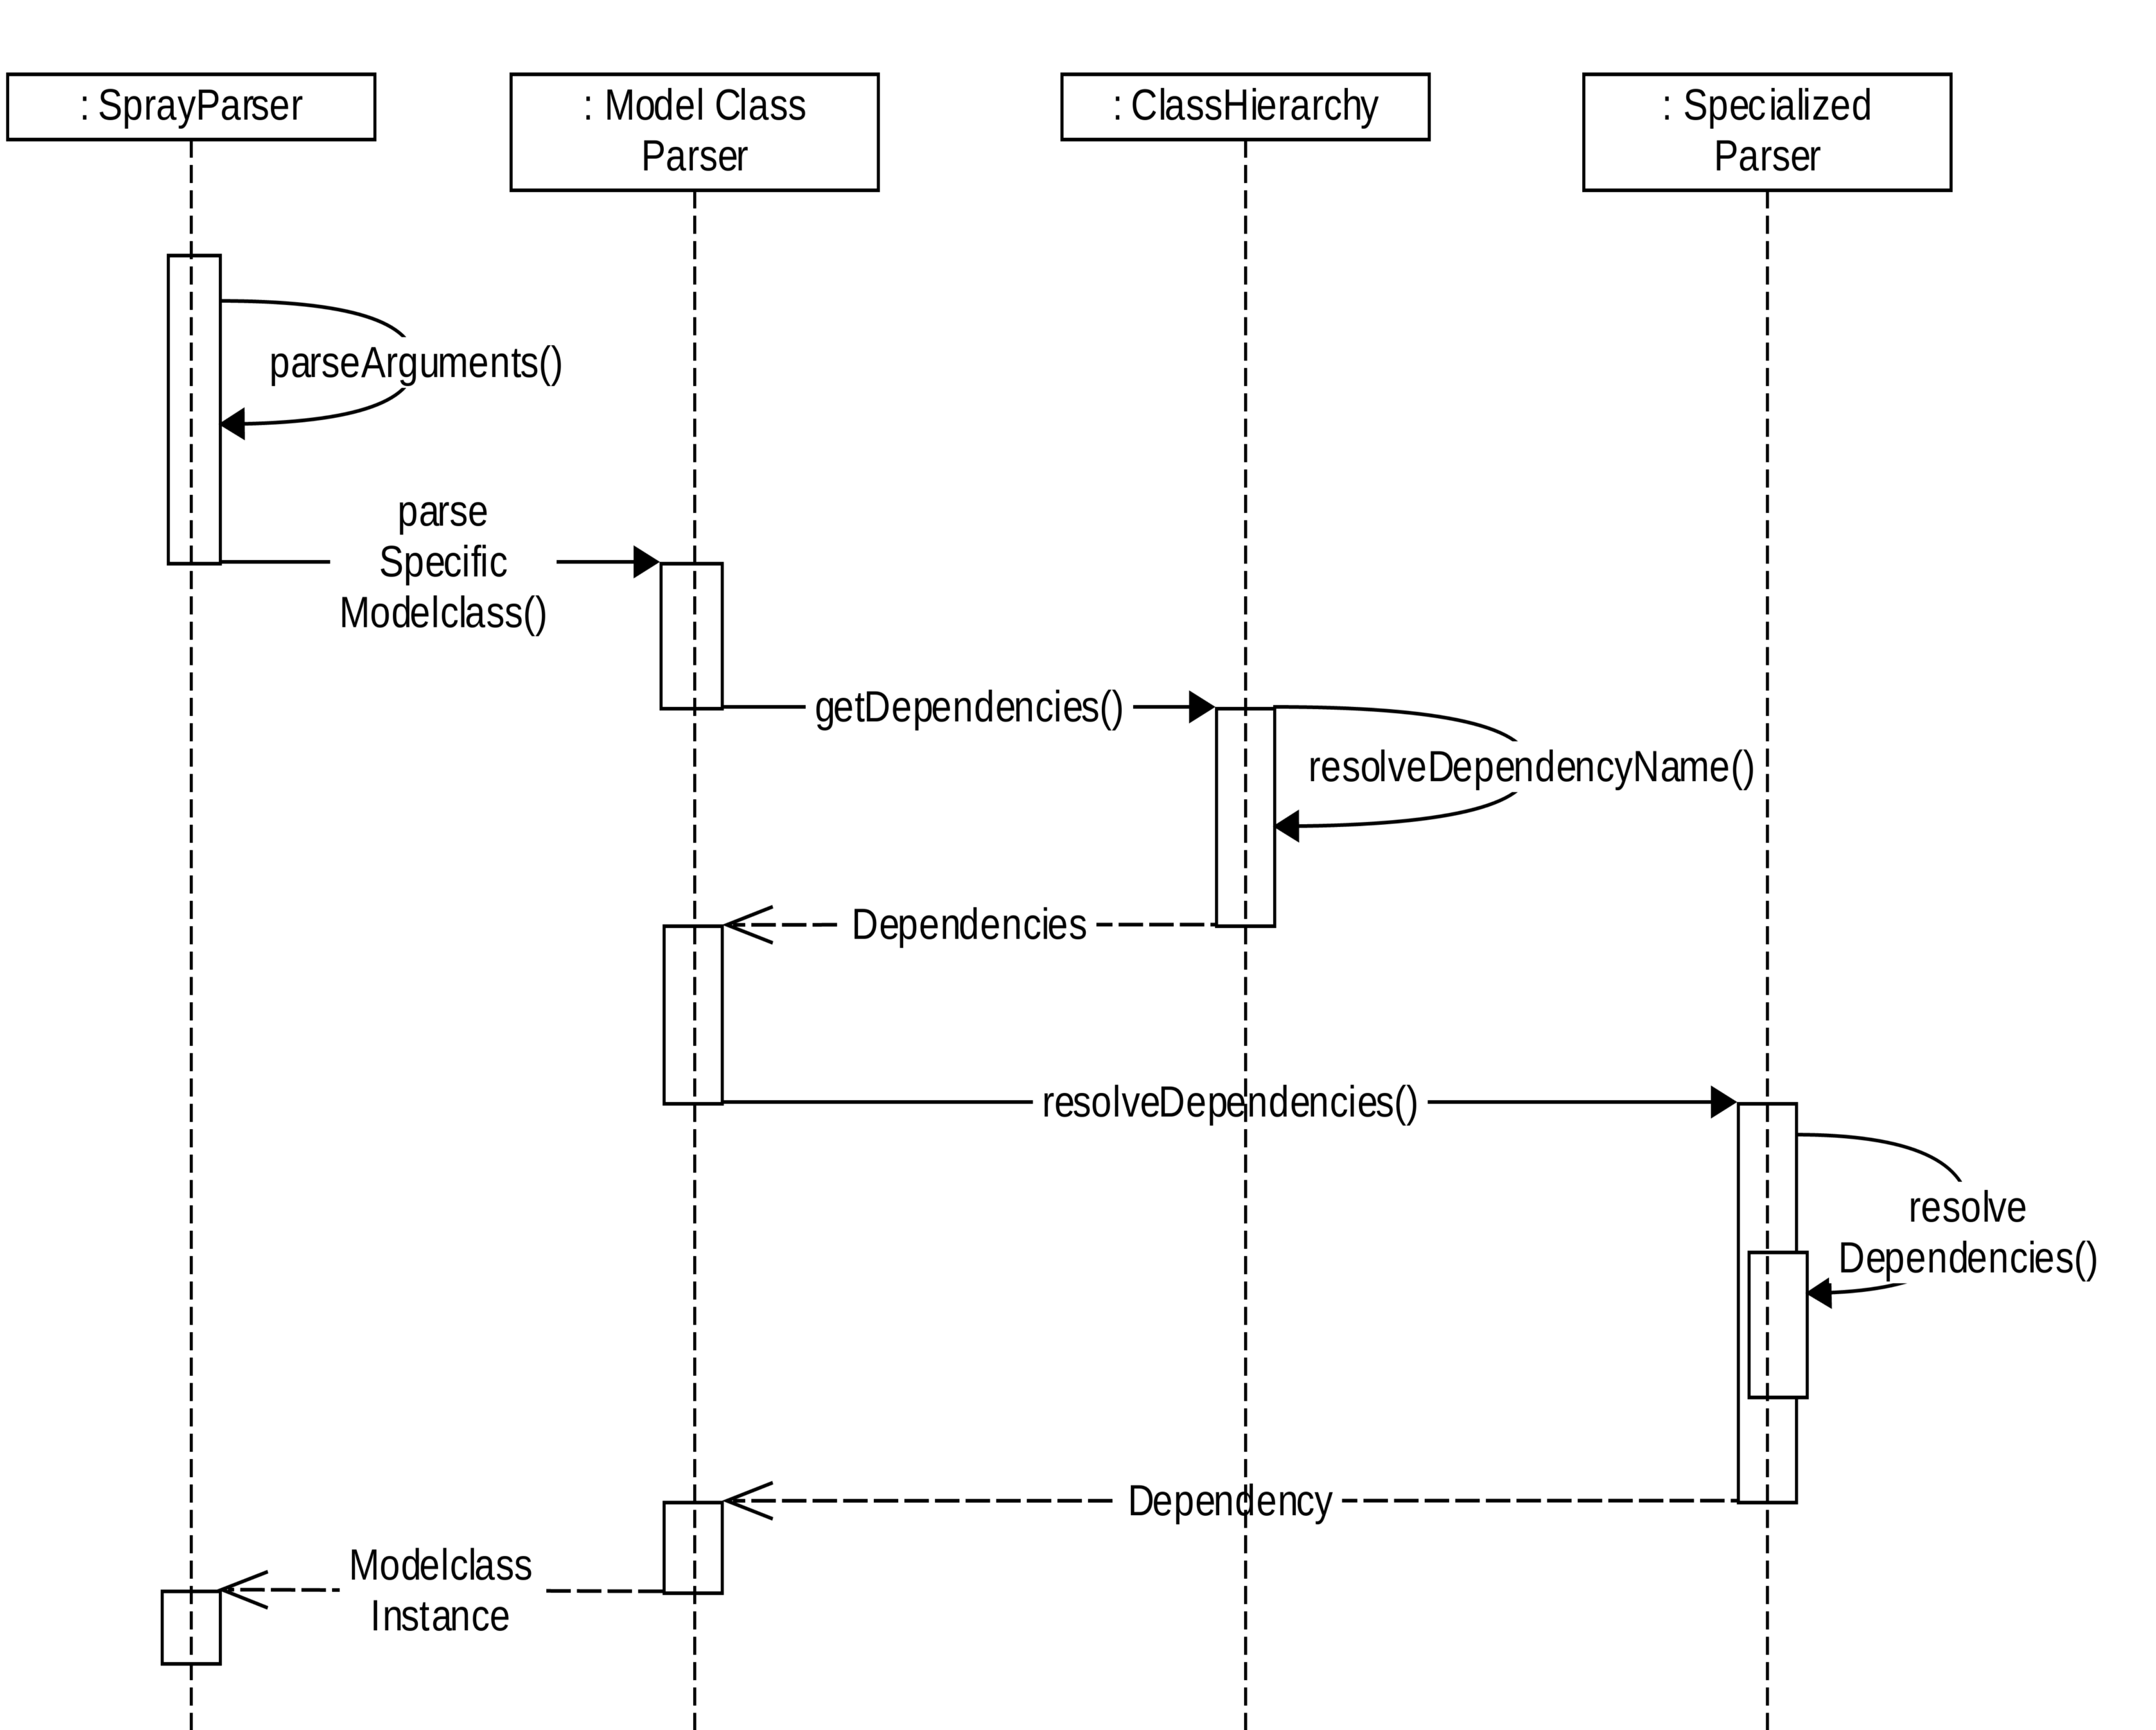
\includegraphics[scale = 0.13]{Bilder/sequenzdiagrammAnsatzKomprimiertScaled(2500x2500).png}
		\caption{Sequenzdiagramm für den Ablauf eines Parsing Vorgangs}
		\label{sequenzdiagrammAnsatz}
\end{figure}Erhält die Applikation einen String um beispielsweise eine Shape einzulesen, werden zunächst sämtliche Attribute aus dem String gefiltert. Hierzu zählen auch Name und erweiterte Shapereferenzen. Dies wird über eine Methode namens \textit{parseArguments}(siehe Abbildung \ref{sequenzdiagrammAnsatz}) erfolgen. Egal um welche Modellklasse es sich handelt, werden alle ausgelesenen Attribute in Stringform weiterverarbeitet. So wird die Verantwortung der Auflösung auf die einzelnen Parser der Modellklassen ausgelagert und diesen gleichzeitig ein einheitliches Medium geliefert. Auf diese Weise können ähnliche oder gleiche Attribute in unterschiedlichen Parsern, auf die selbe Weise aufgelöst werden. Wie bereits angedeutet, geht es von hier an mit einem auf die Modellklasse spezialisierten Parser weiter, der \textit{ModelClassParser}(siehe Abbildung \ref{sequenzdiagrammAnsatz}). Der spezifische Modellklassenparser muss nun zunächst prüfen, ob weitere Instanzen, des Zieltyps erweitert werden sollen. Hierfür gibt er die in den Attributen enthaltene Liste an Eltern (in Form von Strings) an die \textit{ClassHierarchy} weiter, die den Überblick über die Vererbungshierarchie hat und die Namen über ein internes Mapping auf bestehende Referenzen auflösen kann (\textit{resolveDependencyName}, vgl. \ref{sequenzdiagrammAnsatz}). Sind alle Elternteile aufgelöst, kann der modellklassenspezifische Parser nun anhand einer kompletten Liste an Attributen beginnen, die in Stringform enthaltenen Informationen der Abhängigkeiten aufzulösen.
Falls es sich bei den in Stringform enthaltenen Informationen nicht um primitive Datentypen, sondern um komplexe eventuell ineinander geschachtelte Elemente handelt, werden diese wiederum an ihren speziell definierten Parser weitergegeben (\textit{resolveDependencies}, vgl. \ref{sequenzdiagrammAnsatz}). Da die Elemente wie bereits erwähnt eventuell ineinander verschachtelt sind, können viele weitere rekursive Aufrufe auf spezialisierte Parsereinheiten erfolgen, bis schließlich alle Argumente aufgelöst sind und eine fertige Instanz an den \textit{SprayParser} zurück geliefert werden kann.\\\\Die Parserlogik teilt sich also auf viele kleine spezialisierte Parser auf. Dabei gibt es einerseits den \textit{SprayParser}, der die Schnittstelle zu allen vorhandenen Parsern darstellt. Außerdem die vier spezialisierten Style-, Shape-, Connection- und Diagramparser, die die Modellklassen erzeugen und einige weitere kleinere Parser, welche dafür verantwortlich sind, eigens erstellte Datentypen parsen und erzeugen zu können, wie zum Beispiel \textit{Anchors}. 
\section{Auflösung von Vererbungshierarchien}
Ist eine Technik gefunden, mit der sich die DSL in die Objektstruktur der Modellklassen umwandeln lässt, muss direkt die Problematik der Vererbung betrachtet werden, da die hierfür benötigten Techniken schon beim Parsen relevant sind. Es soll ein Vererbungsmechanismus implementiert werden. Entgegen der geläufigen Definition der Vererbung, handelt es sich hierbei nicht um das Erweitern von Klassen, so wie man es aus diversen Programmiersprachen kennt. Die Anforderung definiert, dass einzelne Instanzen der Modellklassen in der Lage sein sollen, Objekte der selben Klasse erweitern zu können. Genauer bedeutet dies, dass eine Instanz \textbf{nicht} in der Lage sein soll dynamisch komplett neue Attribute zu definieren, sondern \textbf{bekannte} Attribute von Elterninstanzen zu übernehmen, beziehungsweise zu überschreiben. "`Erweitern"' soll in diesem Kontext also zwei Situationen beschreiben:
\begin{itemize}
\item Elternteil verfügt über Attribute, die in der erweiternden Klasse nicht vorhanden sind -\textgreater Wert wird geerbt
\item Elternteil verfügt über Attribute, die in der erweiternden Klasse vorhanden sind -\textgreater ignoriere/überschreibe den Wert der erweiterten Klasse
\end{itemize}
Das folgende Beispiel soll verdeutlichen, was gemeint ist:
Es wird eine vereinfachte Style Klasse definiert (Listing \ref{lst:beispielstylevereinfacht}).
\begin{lstlisting}[style=scala, caption = {vereinfachte Style Klassendefinition}, label = {lst:beispielstylevereinfacht}]
class Style(val name:String, val transparency:Double, val line-width:Int)
\end{lstlisting}Nun wird eine Instanz \textit{S1} der Modellklasse über die DSL definiert, welche sowohl einen Namen, als auch eine Angabe zur \textit{transparency} hat (Listing \ref{lst:s1}).
\begin{lstlisting}[style=spray, caption = {Style S1}, label = {lst:s1}]
style S1 {
    transparency = 0.5
}
\end{lstlisting}Eine weitere Instanz \textit{S2} wird definiert, die ihrerseits über einen Namen und eine Angabe zur \textit{line-width} verfügt. Außerdem soll \textit{S2} die Instanz \textit{S1} erweitern:
\begin{lstlisting}[style=spray, caption = {Style S2}, label = {lst:s2}]
style S2 extends S1{
    line-width = 10
}
\end{lstlisting}
Nach dem Parsen dieser Definitionen sollten Objekte folgender Struktur entstanden sein (siehe Listing \ref{lst:s1s2json}).
\begin{lstlisting}[style=spray, caption = {\textit{S1} und \textit{S2} Objekte (aus Gründen der Lesbarkeit aufgeführt in der \textit{Java Script Object Notation})}, label = {lst:s1s2json}]
{
 "name": "S1",
 "transparency": 0.5,
 "line-width":"notDefined"
}

{
 "name": "S2",
 "transparency": 0.5,
 "line-width": 10
}
\end{lstlisting}Wie man sieht verfügt \textit{S2} über eine \textit{transparency} Angabe, die von S1 übernommen wurde. \textit{S1} hat von keiner Seite eine Angabe zur \textit{line-width} bekommen. Unternimmt man an dieser Stelle Überlegungen zur Implementierung, wird man mit folgenden Fragen konfrontiert:
\begin{itemize}
\item Wie weiß ein Objekt, dass es das Attribut des Elternteils übernehmen oder überschreiben soll?
\item Übernimmt S2 tatsächlich alle Attribute des Elternteils oder hält es nur eine Referenz auf S1?
\end{itemize}Die meisten der Attribute, die in der Definition einer Modellklasse berücksichtigt werden können, sind optional. Wie man bei der Definition von S1 sieht, wurde keine Angabe zur \textit{line-width} gemacht. Da die Definition jedoch auf den Konstruktor der Style Klasse abgebildet wird, muss irgendwo eine konkrete Angabe zu dem \textit{line-width} Attribut erfolgen. Man könnte sich überlegen, jedem Feld der Modellklassen einen Defaultwert zuzuweisen. Das bedeutet, dass die \textit{line-width} beispielsweise standardmäßig auf 10 gesetzt wird, wenn in der Definition keine Angabe darüber gemacht wird. Hat aber folglich jede Style Instanz zu jedem möglichen Attribut eine valide Angabe, fragt sich, woher später bekannt ist, ob auf Attribute einer Elterninstanz oder auf die eigenen zugegriffen wird. Immerhin gibt es zu jedem Feld der Instanz gültige Werte.
\subsection{Kennzeichnung nicht definierter Felder in Modellklassen}
Da Integer werte ausschließlich gültige Werte haben, ist es sinnlos 0 als \textit{nicht gesetzt} zu verwenden und 1 - \textit{MAX\_INT} als \textit{gesetzte Werte}. Am Beispiel der \textit{line-width} Angabe in S1 wird also klar, dass bekannt sein muss, ob die Definition den Wert beschreibt oder nicht. 
Deshalb werden alle Felder der Modellklassen (Style, Shape, Connection, Diagram), die ein konkretes Attribut der Modellklasse darstellen, als sogenannte \textit{Options} definiert. Options sind dem Paradigma der funktionalen Programmierung zu verdanken(z.B. in Haskell -\textgreater Maybe).
Sie lösen ein Problem, welches in Java meist mit einer Exception gelöst wird.
Eine Funktion gibt nicht immer für jedes Argument ein gültiges Ergebnis zurück (vgl. \Myciten{esser:scala}{102}). Im Falle der optional setzbaren Attribute der Modellklassen, bieten Options daher die passende Lösung. Man kann sie entweder auf \textit{None} initialisieren oder auf ein \textit{Some$[$T$]$ }. Repräsentativ steht also in diesem Fall \textit{None} für: "`nicht gesetzter Wert"' (schau in den Elternklassen nach entsprechenden Werten) und \textit{Some$[$T$]$} für: "`gesetzter Wert"', ignoriere/überschreibe den Wert der Elternklasse.
\subsection{Vererbungsmechanismus über Referenz auf Elterninstanzen}
Als nächstes ist es derzeit auch noch unklar an welcher Stelle dieser Gedanke Anwendung findet. Es besteht einerseits die Möglichkeit, erst beim unmittelbaren Zugriff auf die einzelnen Felder zu prüfen, ob sie definiert wurden. Andererseits könnten jegliche Elterninstanzen schon bei der Erzeugung einer neuen Instanz nach fehlenden Werten durchsucht werden. Genauer ist also die Frage, ob Modellklassen eine zusätzliche Referenz auf Elternteile erhalten und nicht definierte Werte erst bei Bedarf in den Attributen der Elternliste gesucht werden oder ob Modellklassen schon bei der Instantiierung über sämtliche Attribute der Eltern Bescheid wissen, diese auf sich übertragen und anschließend nicht mehr auf ihre Eltern angewiesen sind. Beide Möglichkeiten bieten Vor- und Nachteile. Referenzen erlauben es, die Extraktionslogik der Attribute auf eine beliebige Stelle im Code auszulagern, je nach dem wann der Aufruf erfolgen soll. 
\subsection{Vererbungsmechanismus durch direkte Weitergabe der Attribute bei Instantiierung}
Werden die Attribute der Elternklasse jedoch direkt bei der Objekterzeugung an die neue Instanz weitergegeben, hat dies zwei besondere Vorteile. Je nach Größe der Vererbungshierarchie ist es wesentlich performanter, die Werte im aktuell benutzten Element zu suchen, als über eine Referenz in den vielen Elternknoten ausfindig zu machen. Außerdem beseitigt diese Vorgehensweise die Rekursivität der Problemstellung.\\\\Dazu ein stark vereinfachtes Beispiel:\linebreak Werden mehrere Modellklassen definiert (siehe Listing \ref{lst:allthestyles}), welche den jeweiligen Vorgänger erweitern und wird davon ausgegangen, dass die Attribute der zu erweiternden Instanzen direkt bei der Erzeugung übernommen werden,
\begin{lstlisting}[style=spray, caption = {Definition einiger Styles, die vom jeweils nächsten Style erweitert werden}, label = {lst:allthestyles}]
style S1 {}
style S2 extends S1 {}
style S3 extends S2 {}
style S4 extends S3 {}
\end{lstlisting}kann davon ausgegangen werden, dass \textit{S2} jedes Element von \textit{S1} erbt, \textit{S3} jedes Element von \textit{S2} erbt und somit auch implizit jedes Element von \textit{S1} usw. Der Reihe nach werden die einzelnen Styles erzeugt. Wird \textit{S2} erzeugt erbt es direkt alle Attribute von \textit{S1}, die es nicht selbst definiert (und somit gegebenenfalls überschreibt). Wird nun \textit{S3} erzeugt, erbt dieser Style nicht mehr direkt von \textit{S1}, da \textit{S2} garantiert alle Felder von \textit{S1} übernommen oder überschrieben hat. So muss bei der Vererbung also immer nur auf die nächst höhere Elterninstanz zugegriffen werden. Diese Eigenschaft lässt sich auf beliebig viele erweiternde Instanzen anwenden, wodurch in dem Beispiel \textit{S4} garantiert jede Eigenschaft von S1, S2 und S3 enthält, oder überschreibt. Da die Rekursivität der Problemstellung so entfällt und den Code (ausschlaggebender Faktor ist die Größe des durch Vererbung erstellten Baumes) performanter gestaltet, wird versucht die Vererbungshierarchie auf diese Weise aufzulösen.

\section{Generatoren}Ausgehend davon, dass nun Strings eingelesen und in entsprechende Instanzen der Modellklassen umgewandelt werden können, ist der nächste Schritt über Generatoren den nun eigentlich gewünschten Code (Generat) zu erzeugen. Hierfür werden entsprechend der Modellklassen einige Generatorenklassen wie z.B. \textit{StyleGenerator} erstellt, welche die Modellklassen in das gewünschte Format umwandeln. Die Generatorenklassen bilden die entstandenen Objektinstanzen auf \textit{Javascript Code} ab.
\chapter{Umsetzung}
Basierend auf den Gedankengängen, die im Ansatz erläutert wurden, wird in diesem Kapitel die Umsetzung beschrieben. Hierbei werden zuvor getroffene Entscheidungen oftmals revidiert und neue Entschlüsse getroffen.
\section{Objektstruktur}
\subsection{Modellklassen}
Da bevor jeder anderer Logik zunächst die zu verwendenden Klassen definiert werden müssen, sollen Diese auch zuerst vorgestellt werden.\\\\Die Modellklassen Style, Shape, Connection und Diagram sind entgegen des Ansatzes, diese als \textit{case classes} umzusetzen, als normale Klassen implementiert worden. Dies hängt damit zusammen, dass die Parserlogik auf verschiedene Einzelparser aufgeteilt wurde.
Entgegen der Objektstruktur, die durch die DSL in Xtext beschrieben wird, mussten einige Beziehungen geändert werden (siehe Abbildungen \ref{objectstructureStyle}, \ref{objectstructureShape}, \ref{objectstructureDiagram}).
Die Xtext Grammatik definiert zwar, welche Elemente nur Definitionsregeln sind und was in die Objektstruktur aufgenommen wird, jedoch liegt es letztlich beim Entwickler zu entscheiden, was in die endgültige Objektstruktur übernommen wird und was nicht.
\subsection{Besonderheiten bei Style}\label{specialstyle}
Bei der Umsetzung der einzelnen Modellklassen aus der Xtext Grammatik in die Objektstruktur in Scala, kam es regelmäßig zu Situationen, in denen die Objektstruktur nicht 1:1 auf Scala übernommen werden konnte, da die verschiedenen Sprachen verschiedene Features bedienen, oder eben nicht (z.B. Xtext Schlüsselwort dispatch). Außerdem galt es bestehende komplexe Strukturen möglicherweise vereinfacht umzusetzen. Beispielsweise enthält die Definition der Style klasse in Xtext ein Style Layout, welches die eigentlichen Attribute der Style klasse auflistet (siehe Listing \ref{lst:xtextdsl}).\\\\
\begin{lstlisting}[style=spray, caption={stark vereinfachter Auszug aus der Xtext Grammatik, die Styles beschreibt}, label = {lst:xtextdsl}]
Style:
    {Style}
    [...]
    layout=StyleLayout
    [...]
;
	
StyleLayout: 
    {StyleLayout}
    (
        ("transparency" "=" transparency=DOUBLE)? &
        [...]
    )
;
\end{lstlisting}
In diesem Fall wurden alle Attribute eines Styles direkt in der Style klasse aufgelistet. Dies vereinfacht einerseits die Objektstruktur, außerdem erleichtert es den Zugriff auf die Attribute, da die Navigation durch die referenzierte Instanz eines Layouts entfällt. Des weiteren definiert die Xtext Grammatik nicht eindeutig um welche Abstraktionsform es sich bei manchen Definitionen handelt (siehe Listing \ref{lst:colororgradient}).
\begin{lstlisting}[style=spray, caption = {Auszug aus der Style.xtext Grammatik, Definition der ColorOrGradient}, label = {lst:colororgradient}]
ColorOrGradient: Color | Transparent | GradientRef
\end{lstlisting}
Also kann an Stelle eines \textit{ColorOrGradient} sowohl eine \textit{Color}-, \textit{Transparent}- oder \textit{GradientRef} Definition stehen. Für das Einbetten in eine Objektstruktur sind diese Regeln nicht ideal, da \textit{Color}, \textit{Transparent} und \textit{GradientRef} keine gemeinsamen Eigenschaften haben. Sie lassen sich zwar unter einer gemeinsamen Abstraktion zusammenfassen, dies bereitet jedoch später im Generator Probleme. \textit{Highlighting} Attribute sind beispielsweise vom Typ \textit{ColorOrGradient}. Später im Generator werden für verschiedene Untertypen von \textit{ColorOrGradient} einheitliche \textit{Getter} Methoden definiert (dies funktioniert in Xtext über eine sogenannte \textit{dispatch} Kennzeichnung), jedoch geht \textit{Gradient} dabei leer aus. Wird also ein \textit{Gradient} definiert, muss der Entwickler blind vertrauen, dass es nicht an der falschen Stelle eingesetzt wurde. Gibt man einem \textit{highlighting} Attribut ein \textit{Gradient}, was laut Abstraktion möglich ist, wird in diesem Fall die Methode \textit{createColorValue} in einem \textit{Gradient} gesucht, welche diese Methode \textbf{nicht} beschreibt. Entwickler müssten also jedes mal wenn die entsprechende Methode aufgerufen wird, zunächst prüfen um was für eine konkrete Unterklasse von \textit{ColorOrGradient} es sich handelt.
Für die Vereinheitlichung der Klassen wurden Traits benutzt. Ausdrücke wie in Listing \ref{lst:xtextmehrfachvererbung}
\begin{lstlisting}[style=spray, caption = {Auszug aus der Style.xtext Grammatik, Color kann als ColorOrGradient oder als ColorWithTransparency benutzt werden}, label = {lst:xtextmehrfachvererbung}]
ColorOrGradient: Color | Transparent | GradientRef;
ColorWithTransparency: Color | Transparent;
\end{lstlisting}zeigen, dass Xtext eine Art der Mehrfachvererbung zulässt. \textit{Color} kann sowohl als \textit{ColorOrGradient}, als auch \textit{ColorWithTransparency} benutzt werden.
Traits haben die Möglichkeit in eine Klasse "'hineingemischt"' (vgl. \Myciten{esser:scala}{191}) zu werden und sollen in diesem Sinne in der Regel weitere Eigenschaften hinzufügen. Hierüber wird das Problem der vermeintlichen Mehrfachvererbung gelöst, da beliebig viele Traits in die Klasse hineingemischt werden können.
Einige Elemente wie zum Beispiel Farbkonstanten ("'light-orange"' -\textgreater LIGHT\_ORANGE, "'blue"' -\textgreater BLUE), wurden nicht wie in Xtext als Enumeration verwirklicht, sondern als \textit{case objects} (siehe Listing \ref{lst:caseobjects}).
\begin{lstlisting}[style=scala, caption = {Auszug aus Code ColorConstants als case objects}, label = {lst:caseobjects}]
case object WHITE      extends ColorConstant {def getRGBValue = """#ffffff""" }
case object LIGHT_GRAY extends ColorConstant {def getRGBValue = """#d3d3d3""" }
case object GRAY       extends ColorConstant {def getRGBValue = """#808080""" }
case object DARK_GRAY  extends ColorConstant {def getRGBValue = """#a9a9a9""" }
...
\end{lstlisting}Da Farbkonstanten (\textit{ColorConstant}) so von Superklassen erben können, ist es möglich einheitliche Methoden für sie zu definieren.
Beispielsweise ist die Methode \textit{createOpacityValue} in einer Superklasse einheitlich beschrieben worden (siehe Listing \ref{lst:traitColor}).\begin{lstlisting}[style=scala, caption = {Auszug aus Code Trait ColorOrGradient}, label = {lst:traitColor}]
trait ColorOrGradient{
   def getRGBValue:String
   def createOpacityValue:String = "1.0"
}
\end{lstlisting}Da ColorOrGradient ein Trait ist, erlaubt es (anders als Javas \textit{Interfaces}), die Methoden vorzuimplementieren. So ist automatisch jede Farbkonstante bedient und es muss nicht erneut wie in Xtext auf eine Weise wie \textit{dispatch} gearbeitet werden.\\\\In Abbildung \ref{objectstructureStyle} ist eine vereinfachte Version der entstandenen Objektstruktur zu sehen, die die wichtigsten Abhängigkeiten der Style Modellklasse darstellt.
\begin{figure}[H]
\begin{center}
\includegraphics[width=\textwidth]{Bilder/styleObjektstruktur.png}
\caption{Vereinfachte Objektstruktur. Im Fokus Style und seine wichtigsten Abhängigkeiten.}
\label{objectstructureStyle}
\end{center}
\end{figure}
\subsection{Besonderheiten bei Shape}
Für Shapes muss zunächst ein Namensproblem aufgelöst werden. Mit einer Shape wird der Wrapper definiert, der sowohl Metainformationen zu der Shape enthält als auch die \textbf{eigentlichen Shapes}, in diesem Fall geometrische Figuren (\textit{GeometricModel}), enthält. Ist also die Rede von GeometricModels, sind die tatsächlichen Implementierungen beispielsweise einer Ellipse gemeint. Ist die Rede von einer Shape, ist die Wrapper Klasse gemeint, welche beispielsweise Ellipsen beinhalten kann. Da die verschiedenen geometrischen Figuren einheitlich behandelt und verwaltet werden können müssen, bildet GeometricModel ihre gemeinsame Abstraktion (siehe Abbildung \ref{objectstructureShape}). Die konkreten geometrischen Figuren haben zwar untereinander hin und wieder Gemeinsamkeiten, doch es lassen sich tatsächlich keine allgemeinen Ähnlichkeiten feststellen. Beispielsweise haben einige zwar Angaben zur Größe, jedoch nicht alle. Aus diesem Grund definiert die abstrakte Klasse GeometricModel lediglich eine Gemeinsamkeit, die für die Distribution von vererbten Informationen wichtig ist: Die Referenz auf ein eventuell existierendes Elternteil. Ein Rechteck, kann ein Polygon beinhalten, welches wiederum ein weiteres Rechteck beinhalten kann (siehe Listing \ref{lst:ellipserectangle}).
\begin{lstlisting}[style=spray, caption = {Beispiel Ellipse die einer Styleregel unterliegt und ein Rechteck beinhaltet}, label = {lst:ellipserectangle}]
ellipse style StandardStyle {
    rectangle {
        ...
    }
}
\end{lstlisting}
In diesem Falle muss garantiert werden können, dass auch das verschachtelte Rechteck über die Style-Attribute der Ellipse verfügt.
Die Layouts der einzelnen geometrischen Formen wurden als Traits realisiert. Der große Vorteil der Traits als \textit{rich-Interfaces} liegt darin, dass mehrere Eigenschaften(Traits) geerbt werden können. So kann jede geometrische Figur von der abstrakten Klasse GeometricModel erben und gleichzeitig die Eigenschaft eines spezifischen Layouts besitzen.
Die Layouts selber haben wiederum nur eine Gemeinsamkeit, nämlich die Möglichkeit einen Style zu referenzieren. Diese Eigenschaft wurde in in dem Trait \textit{Layout} bestimmt, von dem \textbf{jedes} weitere Layout erbt (siehe Abbildung \ref{objectstructureShape}). Da die geometrischen Figuren nun keine Referenz mehr auf Layout Objekte haben, sondern entsprechende Felder selber erben, ist auch hierbei der Navigationsaufwand deutlich verringert. Wenn ein \textit{roundedRectangle} zuvor auf seine Positionskoordinaten zugreifen wollte, gelang dies wie in Listing \ref{lst:navigationsucks}.
\begin{lstlisting}[style=scala, caption = {Beispielnavigation durch komplexe Objektsruktur}, label = {lst:navigationsucks}]
val x_coord = rr.layout.common.x
\end{lstlisting}Durch die Vereinfachung der Objektstruktur und die Umsetzung der Layouts als Traits, können diese Informationen direkt abgerufen werden, sind aber logisch weiterhin von der erbenden Klasse getrennt und können einheitlich gewartet werden. In Abbildung \ref{objectstructureShape} ist eine vereinfachte Version der entstandenen Objektstruktur zu sehen, die die wichtigsten Abhängigkeiten der Shape und Connection Modellklassen darstellt.
\begin{figure}[H]
\begin{center}
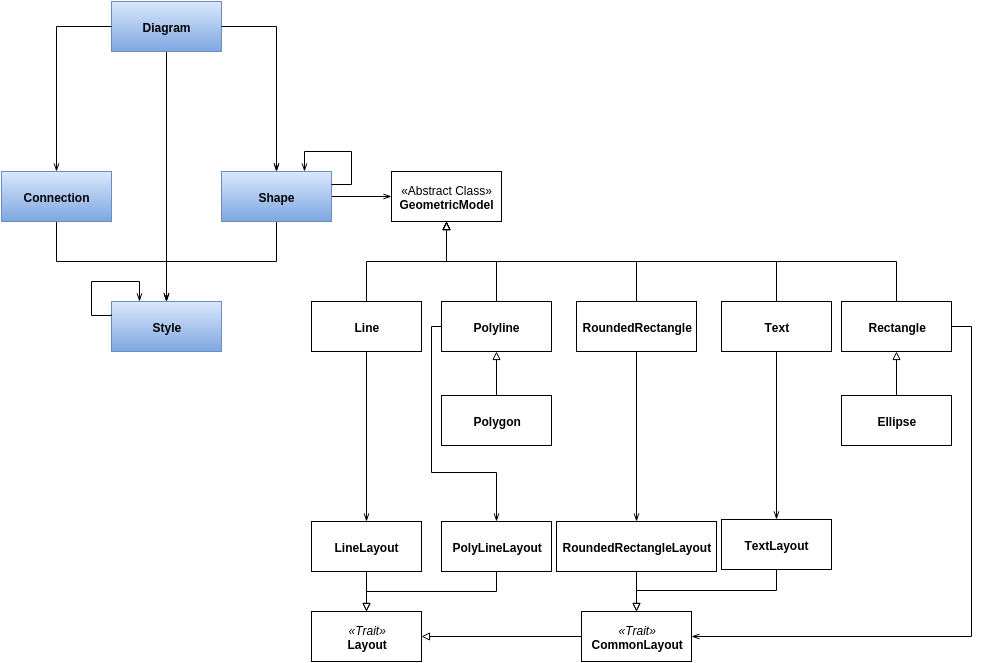
\includegraphics[width=\textwidth]{Bilder/shapeObjektstruktur.png}
\caption{Vereinfachte Objektstruktur. Im Fokus Shape und seine wichtigsten Abhängigkeiten.}
\label{objectstructureShape}
\end{center}
\end{figure}
%\subsection{Besonderheiten bei Connection}
\subsection{Besonderheiten bei Diagram}
Die DSL, in der Diagrams geparst werden, verknüpft das Metamodell und die Modellklassen. Die Definition eines Diagrams sieht (vereinfacht) aus wie in Listing \ref{lst:diagramdefinitionexample}.
\begin{lstlisting}[style=spray, caption = {Beispielhafte Diagram Definition (vereinfacht)}, label = {lst:diagramdefinitionexample}]
diagram diagramName for metamodelElement (style: styleName){
	...
}
\end{lstlisting}Diagrams und einige seiner Attribute verweisen auf ein Metamodell oder dessen Felder, aus dem MoDiGen Projekt.
Da das Metamodell zur Zeit der Entwicklung noch nicht bereit war, wurden diese Elemente mit Mockups versehen (siehe Listing \ref{lst:mclassmock}).
Ein Auszug aus dem SprayParser:\\\\\\\\\\\\
\begin{lstlisting}[style=scala, caption = {Auszug aus Code MclassMock über dass eigentliche MClass Elemente gemockt werden}, label = {lst:mclassmock}]
trait MclassMock {
  var name:String
  def superTypeOf(childClass:MclassMock):Boolean = true
  ...
}
\end{lstlisting}Bemerkenswert ist bezüglich des Zugriffs auf das Metamodell an dieser Stelle, dass Zugriffe auf einzelne Elemente des Metamodells im Gegensatz zu Xtext sehr einfach gestaltet werden können. Dieser Vorteil gegenüber Xtext rührt nicht allein durch Scala, sondern der Entscheidung Metamodelle in der \textit{\textbf{J}ava \textbf{S}cript \textbf{O}bject \textbf{N}otation} in einer \textit{NoSQL} Datenbank zu hinterlegen. Xtext benutzt \textit{XML} (\textit{E\textbf{X}tensible \textbf{M}arkup \textbf{L}anguage}) Dateien als Speichermedium. Zugriff auf spezifische Elemente erfolgt in Xtext über das Laden der gesamten XML Datei (vgl. \Myciten{gunderloy:xml}{58-60}). Da die Entitäten der Metamodelle in MoDiGen einzeln im \textit{JSON} Format in eine \textit{NoSQL} Datenbank eingespeist werden, ist es auch möglich, einzeln auf entsprechende Elemente zuzugreifen. Diese Möglichkeit des Datenzugriffs vermeidet (abhängig von der Dateigröße) unter Umständen riesigen Overhead und ist auf Grund der geringeren Bandbreitenauslastung auch wesentlich performanter. In Abbildung \ref{objectstructureDiagram} ist eine vereinfachte Version der entstandenen Objektstruktur zu sehen, die die wichtigsten Abhängigkeiten der Diagram Modellklasse darstellt.
\begin{figure}[H]
\begin{center}
\includegraphics[width=\textwidth]{Bilder/diagramObjektstruktur.png}
\caption{Vereinfachte Objektstruktur. Im Fokus Diagram und seine wichtigsten Abhängigkeiten.}
\label{objectstructureDiagram}
\end{center}
\end{figure}
\subsection{Vererbung/ClassHierarchy}
Nachdem die Modellklassen definiert wurden, müssen diese wie bereits beschrieben auch hinsichtlich der Vererbungshierarchie verwaltet werden können. Entsprechend des Ansatzes wurde - wie ursprünglich geplant - eine generische Klasse namens \textit{ClassHierarchy} erstellt, welche sowohl Knoten definiert,
als auch eine Map führt, die Namen (Strings) auf entsprechende Knoten abbildet.
Da diese Klasse im Stande sein soll, die Namen, also die tatsächlichen String  Attribute der Style- und Shape Klassen abzubilden, wurde in der Typparameterliste ein \textit{Viewbound} definiert (siehe Listing \ref{lst:viewbound}).
\begin{lstlisting}[style=scala, caption = {Auszug aus Code Viewbound. Implizite Umwandlung auf { val name:String}}, label = {lst:viewbound}]
sealed class ClassHierarchy[T <% {val name:String}](rootClass:T){
\end{lstlisting}Die Kennzeichnung \textit{ X \textless\% Y} sagt aus, dass der übergebene Typ \textit{X} implizit auf den Typ \textit{Y} umgewandelt werden können muss (vgl. \Myciten{braun:scala}{158}).
In Diesem Fall wurde ein anonymer Typ erstellt, der ein Feld \textit{name:String} besitzt. Wenn der angegebene Typ also über ein solches Feld verfügt, kann er implizit darauf abgebildet werden und wird akzeptiert.
Des weiteren wurden mehrere \textit{Apply}-Methoden definiert, die den Umgang mit \textit{ClassHierarchy} erleichtern sollen (siehe Listing \ref{lst:applymethoden}).
\begin{lstlisting}[style=scala, caption = {Auszug aus Code Apply Methoden, die die Benutzung von ClassHierarchy erleichtern}, label = {lst:applymethoden}]
def apply(parent:Node, className:T) =
	parent inheritedBy className
def apply(parent:T, className:T) =
	nodeView(parent.name) inheritedBy className
def apply(parent:String, className:T) =
	nodeView(parent) inheritedBy className
def apply(className:T) =
	nodeView(className.name)
def apply(className:String) = 
	nodeView(className)
\end{lstlisting}Apply-Methoden sind spezielle Methoden und können ohne den eigentlichen Methodennamen aufgerufen werden. Die Argumente werden einfach nach der Instanz in Klammern angegeben (vgl. \Myciten{esser:scala}{74}). Dies ist sehr komfortabel. Eltern- und Kindbeziehungen werden in den Knotenklassen gespeichert. Leider ist \textit{ClassHierarchy} so jedoch, wie sich herausstellt, nicht wie gewünscht einsetzbar.
Wird ein neuer Style oder eine neue Shape erzeugt, müssen die Eigenschaften der Elternknoten verfügbar sein, noch bevor der/die eigentliche Style/Shape instantiiert wurde, da diese Eltern und deren Felder noch vor dem Instantiieren des neuen Objekts aufgelistet und abgerufen werden. Das \textit{Companion Objekt} der entsprechenden Klassen sammelt erst alle Informationen an neu geparsten und an geerbten Attributen und gibt diese dann an den richtigen Konstruktor weiter (siehe Abschnitt \ref{sectionInheritance}). Bevor also ein Style/Shape instantiiert ist, kann in \textit{ClassHierarchy} auch nicht danach gesucht werden, es existiert ja noch nicht. Entsprechende Elternknoten des noch nicht existierenden Knotens sind so ebenfalls nicht ausfindig zu machen. Dieser Denkfehler reduziert die Brauchbarkeit der \textit{ClassHierarchy}-Klasse auf die Map[String, T], welche diese noch enthält. Da die Namen der Elternklassen über die Definition der Modellklasse mitgeliefert werden, werden die Entsprechenden Elternteile über die Abbildung String=\textgreater T der Map gefunden.
Die komplette, gebrauchte Funktionalität der ClassHierarchy ist also bereits durch eine herkömmliche Map der scala.collections beschrieben. Lediglich die zusätzlichen apply-Methoden der ClassHierarchy, welche den Gebrauch der Map vereinfachen, sorgen derzeit dafür, dass die Klasse einen Nutzen erfüllt. Schließlich behalten die erzeugten Styles/Shapes eine Liste mit ihren Eltern. Da sie in sich alle Merkmale der Superklassen behalten, wäre dies nicht einmal nötig. Jedoch bleibt es zu Testzwecken nützlich eine solche Referenz zu haben, um schnell überprüfen zu können welche Werte übernommen wurden, welche nicht und warum nicht (z.B. \textit{latest-bound principle}).
\section{Implementierung der Parserklassen}
Sind die Beziehungen unter den Modellklassen definiert, muss als nächstes dafür gesorgt werden, dass entsprechende Klassen auch instantiiert werden können. Da die benötigte Information für die Erstellung einer Modellklasse in Stringform bereitgestellt wird, ist also nun ein Parser einzurichten, der die benötigte Umwandlung der in Stringform enthaltenen Attribute zu den richtigen Datentypen vollziehen kann.
\subsection{Factory Klassen}
Der Parser muss, dem Metamodell entsprechend, unter anderem sowohl Style-, Shape-, als auch Diagram Definitionen verarbeiten können (siehe Abbildung \ref{diagramshapestyle}). Entsprechend wurden Diagram.scala, Shape.scala und Style.scala erstellt. Zunächst waren diese Klassen als \textit{case classes} geplant, um bestimmte Methoden vorimplementiert benutzen zu können. Allerdings wurde schlussendlich entschieden, Teile der Parserlogik auszulagern. Gemäß dem \textit{Single Responsibility Principle} (vgl. \Myciten{martin:clean}{181}), lag es nahe sowohl einen Style-, Shape- und Diagramparser zu haben, auf die der eigentliche Parser zurückgreifen kann.
Im Idealfall würden diese spezialisierten Parser wie \textit{Factorys} agieren, um die zugehörige Klasse möglichst entkoppelt instantiieren zu können. Die \textit{Factorys} wurden als \textit{Companion Objekte} realisiert, da diese sich hierfür besonders eignen. Diese Absicht kreuzt sich leider mit den \textit{case classes}, da diese bereits implizit über ein \textit{Companion Objekt} verfügen. Diese \textit{Companion Objekte} können nicht partiell überschrieben werden.
Jede der (normalen) Modellklassen hat nun ein \textit{Companion Objekt}, welches eine \textit{parse} Methode enthält, um seine \textit{Companion Klasse} zu instantiieren.
Die \textit{Companion Objekte}, können hierbei als \textit{Factory} angesehen werden, da ihre \textit{apply}-Methoden den Parse Vorgang ebenfalls initiieren und anschließend eine neue Instanz ihrer \textit{Companion Klasse} zurückliefern (vgl.\Myciten{esser:scala}{80}).
Eine Modellklasse kann also erzeugt werden, indem ohne \textit{new} das Companion Objekt mit der entsprechenden Argumentenliste aufgerufen wird.
Die Fabrikmethode bekommt Argumente als Tupel aus Strings Form (z.B. ("'line-width"', "'4"') -\textgreater  Integer 4 wird aufgelöst und anhand des Attributnamens an der richtigen Stelle im Konstruktor platziert) und der eigentliche Konstruktor nur aufgelöste Werte als Argumente akzeptiert.
Das oben beschriebene Prinzip, der Aufteilung der Parserlogik in mehrere kleine Parser, wird konsequent durchgeführt. So haben eigene Datentypen wie z.B. \textit{GradientAlignment}, oder \textit{Anchor} ebenfalls kleine Parsereinheiten in ihren Companion Objekten.
Um sicherzustellen, dass auf eigene Faust keine Modellklasse erzeugt werden kann, wird der Konstruktor auf \textit{private} gesetzt und die Klasse mit \textit{sealed} gekennzeichnet. So ist es ausschließlich über das Companion Objekt möglich eine Modellklasse zu erzeugen. Dem Companion Objekt ist der Zugriff auf den privaten Konstruktor möglich, da es Zugriff auf alle privaten Member der \textit{Companion Klasse} hat. Ansonsten könnten im schlimmsten Fall sogar abstrakte Klassen anonym instantiiert werden (siehe Listing \ref{lst:instantiateabstract}).
\begin{lstlisting}[style=scala, caption = {Beispiel zur Instantiierung der abstrakten Klasse GradientAlignment}, label = {lst:instantiateabstract}]
val gradient_alignment = new GradientAlignment(){}
\end{lstlisting}
Das Schlüsselwort \textit{sealed} verhindert, dass die gekennzeichnete Klasse außerhalb ihrer Quelldatei erweitert werden kann. So wäre es erneut möglich die Klasse um eine Ecke selber zu instantiieren (siehe Listing \ref{lst:instantiateabstractextends}).
\begin{lstlisting}[style=scala, caption = {Beispiel zur Instantiierung der abstrakten Klasse GradientAlignment über Vererbung}, label = {lst:instantiateabstractextends}]
class AnotherGradient extends GradientAlignment

& 
 
val anonymous_gradient = new AnotherGradient()
\end{lstlisting}
Da davon ausgegangen werden kann, dass die Modellklassen nur über geparsten Input erstellt werden können, ist es sicherer auch ihre Instantiierung \textbf{ausschließlich} den Parsern zu überlassen. Deshalb sollten alle Modellklassen auf diese Weise definiert werden.

\subsection{Problematik der rekursiven regulären Ausdrücke}
Das tatsächliche Parsen der Strings, erfolgte zunächst über reguläre Ausdrücke. Warum dies in der Umsetzung scheitert und wie das Problem zu lösen ist, wird in diesem Abschnitt erläutert.\\\\Zunächst erscheint es einleuchtend die Strings über \textit{Regular Expressions} einzulesen und auszuwerten. Ist die zugrundeliegende Grammatik simpel genug, funktioniert dies auch einwandfrei. Simple String \textit{match}-Funktionen lassen sich in Scala sehr viel komfortabler anwenden als beispielsweise in Java. Nun wurde zunächst der Style Parser komplett und fehlerfrei fertig gestellt. Die bestehende Lösung definierte viele undurchsichtige Regeln, nicht zuletzt da komplexe reguläre Ausdrücke einfach nicht schön zu lesen sind. Entsprechend ist die Skalierbarkeit einer solchen Lösung nicht sehr effizient, da um eine ohnehin schon komplexe Regel zu erweitern, erst einmal die bestehende Regel verstanden werden muss, was wie bereits erwähnt nicht trivial ist. Dies kann einige Zeit in Anspruch nehmen. Beim erstellen der Regeln für die Shape Klassen stießen die regulären Ausdrücke endgültig an ihre Grenzen. Vor Allem die Anforderung der DSL, ineinander geschachtelte geometrische Figuren abbilden zu können, ist mit regulären Ausdrücken nicht machbar. Eine Shape Definition wie in Listing \ref{lst:shapeellipseellipse}.
\begin{lstlisting}[style=spray, caption = {Beispielhafte Shapedefinition}, label = {lst:shapeellipseellipse}]
shape exampleShape {
    ellipse {
        size (width=50, height=50)
        ellipse {
            size (width=38, height=38)
        }
    }
}
\end{lstlisting} Die Shape in Listing \ref{lst:shapeellipseellipse} ist einerseits sehr komplex, da man um sie parsen zu können sehr komplizierten und unschönen Code erzeugen muss. Das Problem ist, dass beim Parsen zwar ein "`size(width=50, height=50)"' Attribute ermittelt werden kann, die Zuweisung zur richtigen Ellipse aber höchstens auf einer Indexvariable basieren könnte, die die \textit{size} an Stelle \textit{n}, der geometrischen Figur an Stelle \textit{n} zuweist. Doch hierbei müssten zahlreiche Fälle beachtet werden, zumal nicht für jede geometrische Figur jede mögliche Angabe in der Definition auch erfolgen muss. Das weitaus größere Problem ist,
dass normale reguläre Ausdrücke an rekursiven Ausdrücken scheitern, da Scala (Stand Version 2.11.7) keine rekursiven regulären Ausdrücke unterstützt. Setzt die Grammatik also voraus, dass ein Element \textbf{beliebig} oft in sich selbst gekapselt werden kann (z.B. Listing \ref{lst:babuschka}),
\begin{lstlisting}[style=scala, caption = {Beispiel für eine rekursive Grammatik anhand der russischen \textit{Babuschka} Puppen}, label = {lst:babuschka}]
Babuschka {
    Babuschka {
        Babuschka {}
    }
}
\end{lstlisting}sind reguläre Ausdrücke dem Problem nicht mehr gewachsen.
In diesem Fall muss auf eine komplexere Technologie zurückgegriffen werden.
\subsection{Lösung Parser Combinators}Hierbei bieten sich die \textit{Parser Combinator} Klassen an. Wie der Name schon vermuten lässt, kann man hier Parser zusammenschalten, um so komplexe Ausdrücke auswerten zu können. Hierfür werden Methoden definiert, welche als Rückgabewert einen \textit{Parser$[$T$]$} liefern. Für \textit{Parser} sind unter anderem die Methoden \textit{$\sim$}, \textit{$\sim$\textgreater} und \textit{\textless$\sim$} angegeben, welche sich wie normale Operatoren anfühlen und verwenden lassen. Braun hat dies in seinem Werk \textit{SCALA Objektfunktionale Programmierung} wie folgt einleuchtend erklärt (\Myciten{braun:scala}{182}):
\begin{itemize}
\item \textit{a} $\sim$ \textit{b} erzeugt einen Parser, der zuerst a, dann mit b parst und das Gesamtergebnis zurückgibt.  
\item \textit{a} $\sim$\textgreater \textit{b} parst genauso wie \textit{a} $\sim$ \textit{b}, gibt aber nur das Ergebnis des Parsers \textit{a} zurück.
\item \textit{a} \textless$\sim$ \textit{b} gibt analog nur das Ergebnis von \textit{b} zurück. 
\end{itemize}Zunächst ein einfaches Beispiel in der interaktiven scala \textit{REPL} (siehe Listing \ref{lst:simpleparserexample}), in dem ein Parser namens \textit{NameParser} erstellt wird. Für diesen wird eine Methode \textit{name} definiert, welche aus einem String "`hello my name is \textless name \textgreater"' den entsprechenden Name filtert und zurück liefert.
\begin{lstlisting}[style=scala, caption={Einfaches Beispiel für einen Namens Parser}, label = {lst:simpleparserexample}]
scala> import scala.util.parsing.combinator.JavaTokenParsers
import scala.util.parsing.combinator.JavaTokenParsers

scala> class NameParser extends JavaTokenParsers {
     | def name = "hello my name is" ~> ident ^^ {_.toString}
     | }
defined class NameParser

scala> val p =new NameParser()
p: NameParser = NameParser@2ecaa79e

scala> p.parse(p.name, "hello my name is Julian")
res0: p.ParseResult[String] = [1.24] parsed: Julian
\end{lstlisting}Mit relativ wenig Aufwand können sogar sehr komplexe Grammatiken beschrieben werden (siehe Listing \ref{lst:babuschkaexample}).\\\\\\
\begin{lstlisting}[style=scala, caption={Einfaches Beispiel zum Parsen einer rekursiven Grammatik}, label = {lst:babuschkaexample}]
scala> import scala.util.parsing.combinator.JavaTokenParsers
import scala.util.parsing.combinator.JavaTokenParsers

scala> class BabuschkaParser extends JavaTokenParsers{
	def babuschka:Parser[String]=("babuschka" ~> ident) ~ ("{" ~> (babuschka|"") <~ "}") ^^ {_.toString}
}
defined class BabuschkaParser

scala> val p = new BabuschkaParser()
p: BabuschkaParser = BabuschkaParser@23a1ef14

scala> p.parse(p.babuschka, "babuschka b1{ babuschka b2 {babuschka b3 {babuschka b4{}}}}")
res3: p.ParseResult[String] = [1.36] parsed: (b1~(b2~(b3~(b4~))))
\end{lstlisting}Umgesetzt wurden so beispielsweise die rekursiven \textit{GeometricModels}- geometrische Figuren - welche in sich gekapselt erzeugt werden können (siehe Listing \ref{lst:geometricmodel}).
\begin{lstlisting}[style=scala, caption={Rekursive Methode zum Parsen geometrischer Figuren}, label = {lst:geometricmodel}]
private def geoModel: Parser[GeoModel] =
    geoIdentifier ~
    ((("style" ~> ident)?) <~ "{") ~
    rep(geoAttribute) ~
    (rep(geoModel) <~ "}") ^^ {
      case name ~ style ~ attr ~ children =>
        GeoModel(name, style, attr, children, cache)
      }
\end{lstlisting}Wie man sieht ist die Methode \textit{geoModel} rekursiv, da sie sich selbst aufruft. Doch zunächst erst ein paar einfachere Parser.
\subsection{Prinzip der Parserlogik}Die gewählte Technologie zum Parsen sind also \textit{Parser Combinators}, über welche komplexe Problemstellungen gelöst werden können. Wie die einzelnen Parser untereinander assoziiert sind, was ihre jeweiligen Aufgaben sind und welche Gedanken dahinter stecken wird nun beschrieben.\\\\Die grundlegende Parserinstanz, mit der auch der Benutzer schlussendlich interagiert ist der \textit{SprayParser}. Wie bereits erwähnt, sollte dieser Parser möglichst generisch funktionieren, um das Parsen der verschiedenen Modellklassen im Idealfall möglichst einheitlich gestalten zu können (siehe \ref{ansatzlexer}). Konkret heißt das, dass versucht wurde so wenig expliziten Inhalt der Modellklassen abzufragen wie möglich. Anstatt eine Regel aufzustellen, die also beispielsweise direkt nach einem \textit{line-width} Attribut sucht, wurden Regeln gewählt, die allgemeiner auf die Attribute eingehen (siehe Listing \ref{lst:allgemeineparserregeln}).
\begin{lstlisting}[style=scala, caption = {Auszug aus Code beispielhafte Regeln, die verallgemeinerte Attribut- Wert Tupel parsen}, label = {lst:allgemeineparserregeln}]
def attributePair: Parser[(String, String)] = 
	variable ~ arguments ^^ { case v ~ a => (v, a) }
def variable:Parser[String] =
    "[a-züäöA-ZÜÄÖ]+([-_][a-züäöA-ZÜÄÖ]+)*".r <~ "\\s*".r
def arguments: Parser[String] =
    argument_classic | argument_advanced_explicit | 
    argument_advanced_implicit | argument_wrapped
\end{lstlisting}
Es wird also zunächst definiert, dass beim Parsen von Attributen ein \textit{attributePair} erwartet wird. Dieses \textit{attributePair} besteht aus einer \textit{variable} und (\textasciitilde) \textit{arguments}. Eine Variable wird in der nächsten Regel bzw. Methode definiert.
Die vielen verschiedenen Möglichkeiten den Variablenwert zu ermitteln führt darauf zurück, dass dieser Teil nun eben sehr variabel ist. An dieser Stelle kann jeder dem System bekannte Datentyp folgen. Während ein \textit{argument\_classic} erwartet, dass ein '=' Zeichen und anschließend irgendein Int, double oder String folgt, deckt ein \textit{argument\_advanced\_explicit} die Möglichkeit eines Arguments wie in Listing \ref{lst:argumentexplicit}.
\begin{lstlisting}[style=scala, caption = {Beispiel für eine Attributsdefinition mit expliziter Parameterbenennung}, label = {lst:argumentexplicit}]
someSize ( width = 10, height = 12)
\end{lstlisting}Da diese und weitere Parserregeln öfter gebraucht werden, sind diese in einem Trait namens \textit{CommonParserMethods} zusammengefasst. Die \textit{Companion Objekte} der Modellklassen, die gleichzeitig den Parser bilden, erweitern diesen Trait.
Blickt man zurück auf \textit{attributePair}, sieht man außerdem, dass diese Methode ein \textit{Tupel} zurück gibt, welches eben zum einen den Variablennamen und außerdem den Wert zurückliefert.
Da an dieser Stelle des Parsers noch keiner der Werte in seinen eigentlichen Typ konvertiert wird, kann nun auch ein einheitlich typisiertes Set an Tupel[String, String] an die tiefer liegenden Parser weitergegeben werden.
Wird also gerade beispielsweise ein Style geparsed, werden die erhaltenen Tupel nun an das Companion Objekt \textit{Style} übergeben, das sich selber um seine Attribute zu kümmern hat.
Bisher wurde also nur darauf geachtet, dass der Inputstring möglichst mit keiner Konvention der zugrundeliegenden Grammatik bricht, außerdem wird so ein einheitliches Medium garantiert, nach dem sich die spezialisierten Parser der Modellklassen richten können. Da diese grundlegenden Regeln noch keine konkreten Instanzen erzeugen, sondern nur dem Identifizieren der einzelnen Wörter der DSL und der Bereitstellung einheitlicher Datenformate dient, bildet diese logische Einheit (SprayParser) den \textit{Lexer} der Anwendung (vgl. \Myciten{parsing}{135}).
Da sich die spezialisierten Parser nun ihr Inputformat teilen, können sie folglich auch mit denselben Methoden weiterarbeiten.
So muss das Rad nicht für jeden Parser neu erfunden werden.
Ab jetzt passiert im spezialisierten Style Parser die eigentliche Magie.
Bevor die übergebenen Werte in den Tupeln nun ihre endgültige Form erhalten, widmen sich die \textit{Factorys} zunächst der Vererbung. Dazu mehr in Abschnitt \ref{sectionInheritance}.
Nachdem die vererbten Werte berücksichtigt sind, werden nun die Tupel mit den Attributen auseinandergenommen und vordefinierten Variablen zugewiesen, welche später an den Konstruktor der Modellklasse weitergegeben werden.
Die Factory erhält also ein Set mit Attributen. Diese Attribute sind in Form eines Tupels[String, String] und enthalten jeweils den Namen des zuzuweisenden Feldes und den Attributswert(aber immer in String Form). Um Die Werte aufzulösen und zuzuweisen, wird eine mächtige Technik namens \textit{Pattern Matching} eingesetzt (siehe Listing \ref{lst:patternmatching}).
\begin{lstlisting}[style=scala, caption = {Auszug aus dem Code zum Pattern Matching}, label = {lst:patternmatching}]
attributes.foreach{
    case ("description", x) => 
    	description = Some(x)
    case ("transparency", x) => 
    	transparency = ifValid(x.toDouble)
    case ("line-style", x) => 
    	line_style= LineStyle.getIfValid(x)
    ...
}
\end{lstlisting}
So wird immer zunächst geprüft um welches Feld es sich handelt. Anschließend wird der String falls nötig auf den gewünschten Typ konvertiert und zugewiesen. Da Fehleingaben wie Buchstaben an Stelle einer erwarteten Zahl möglich sind, wird über eine Hilfsmethode \textit{ifValid} (siehe Listing \ref{lst:ifValid}) sichergestellt, dass es nicht zum Programmabsturz kommt, sondern im Fehlerfall ein Defaultwert eingesetzt wird.
\begin{lstlisting}[style=scala, caption = {Auszug aus dem Code Methode ifValid}, label = {lst:ifValid}]
def ifValid[T](f: => T):Option[T] = {
      var ret:Option[T] = None
      try { ret = Some(f)
      ret
      }finally {
        ret
      }
}
\end{lstlisting}Die Methode \textit{ifValid} erwartet einen Typparamter und einen Codeblock, der ein Ergebnis entsprechend des Typparameters zurückliefert. Der gewünschte Codeblock wird in einer sicheren \textit{try} Umgebung ausgeführt. Bei erfolgreicher Ausführung wird das Ergebnis des Codeblocks zurückgeliefert, ansonsten \textit{None}.
Der Aufruf von \textit{ifValid} kann wie man in Listing \ref{lst:patternmatching} sieht, aber sogar ohne Typparameter erfolgen, da Scala diesen auch hier anhand der Zuweisung erkennen kann und ihn inferiert (Scala ist klasse!).
Im Falle der Styles werden größtenteils nur primitive Datentypen geparsed, daher ist das konvertieren der Werte in die eigentlichen Datentypen auch eher einfach.
Im Falle der Shape Modellklasse werden unter anderem mehrere ineinander gekapselte geometrische Formen geparsed. Beim Parsen der Ellipsen, Rechtecke etc. sind mehrere Parser beteiligt. Beim Pattern Matching des Shape Companion Objekts wird daher in der Regel auf weitere spezialisiertere Parser verwiesen (siehe Abbildung \ref{sequenzdiagrammAnsatz}).


\section{Vererbung}\label{sectionInheritance}
Da Styles und Shapes auch mit einem \textit{extends} Schlüsselwort definiert werden können, muss auch ein Mechanismus vorhanden sein, der sich um die Vererbungshierarchie kümmert und die Felder der erweiterten Klassen abrufen kann.
Bisher wurde die Vererbung über eine Referenz zum Elternknoten geregelt. Wenn also ein gefragter Wert in der aktuellen Klasse nicht gefunden wurde, suchte man rekursiv in den Elternklassen danach.
Dies erfordert nun einerseits bei größeren Hierarchien einige Zeit, außerdem eventuell komplizierte rekursive Funktionen.
Ein leichterer und performanterer Weg wurde darin gefunden, die Werte eines Elternknotens direkt beim Erzeugen der neuen Instanz auf das Kind zu übertragen.
In dem Companion Objekt von Style/Shape, in dem die Attribute für einen neuen Style aufgelöst werden, wird hierfür zuerst die Liste an Eltern erstellt (siehe Listing \ref{lst:extendedstyle}).
\begin{lstlisting}[style=scala, caption = {Auszug aus Code sammeln der Elterninstanzen}, label = {lst:extendedstyle}]
val extendedStyle:List[Style] = parents.getOrElse(List()).foldLeft(List[Style]())((styles, s_name) =>
      if(cache.styleHierarchy.contains(s_name.trim)) s_name.trim :: styles else styles)
\end{lstlisting}Dafür wird in der vom Parser mitgegebenen ClassHierarchy (\textit{styleHierarchy}) nach den Namen der Eltern gesucht (wieso hierbei die ClassHierarchy Instanz nicht angesprochen werden muss und warum der Liste aus Styles augenscheinlich immer nur Strings zugewiesen werden, wird in \ref{sectionimplicit} erklärt).
Anschließend werden die verschiedenen Variablen, die später an den Konstruktor übergeben werden vordefiniert (siehe Listing \ref{lst:relevant}).\\\\\\\\
\begin{lstlisting}[style=scala, caption = {Auszug aus Code Zuweisung der Felder der Elternelemente}, label = {lst:relevant}]
var description:Option[String]=relevant{_.description}
var line_color:Option[Color]=relevant{_.line_color}
var line_style:Option[LineStyle]=relevant{_.line_style}
var line_width:Option[Int]=relevant{_.line_width}
\end{lstlisting}Auffällig ist hierbei, dass die Zuweisungen beinahe auch für nicht Programmierer lesbar sind. Wie zum Beispiel die erste Zuweisung in Listing \ref{lst:relevant}: \textit{"'Weise der description die relevante bestehende description zu"'}. Hinter diesem Aufruf verbirgt sich eine Funktion, die in ClassHierarchy definiert wurde, um einfach auf die Attribute der Elternklasse zugreifen zu können (siehe Listing \ref{lst:mostrelevant}).
\begin{lstlisting}[style=scala, caption = {Auszug aus Code Funktion mostRelevant}, label = {lst:mostrelevant}]
def mostRelevant[T, C](stack:List[C])(getter: C => Option[T]):Option[T] = {
    for (parent <- stack) {
      if(getter(parent).isDefined)
        return f(parent)
    }
    None
}
\end{lstlisting}Die Methode \textit{mostRelevant} macht Gebrauch von mehreren nützlichen Eigenschaften von Scala. Zunächst wird die Methode mit Typparametern beschrieben. Was diese jeweils beschreiben sollen wird gleich klar. Sinn und Zweck der \textit{mostRelevant} Methode ist es dem Benutzer zu ermöglichen, einen generischen \textit{getter} auf beliebige Felder der Oberklassen zu bieten. Sowohl Style als auch Shape führen eine Liste mit den Instanzen, die sie erweitern.
Genauer, führen Style und Shape eine Art \textit{Stack}, denn bei der Vererbung soll hier das \textit{latest-Bound-Principle} gelten. Dieser Stack wird als erster Parameter übergeben.
Als nächstes sieht man eine weitere Parameterliste, die eine Funktion erwartet. Da die Funktion komplett typunabhängig funktionieren soll, wurden Typparameter benutzt. C stellt in diesem Fall den Typ der Modellklasse dar, T hingegen ist der Typ des gewünschten Elternattributs. Die Funktion bildet eine Modellklasse (C) auf den gewünschten Typ (T) ab und ist somit als \textit{Getter} Methode zu verstehen. 
\textit{MostRelevant} iteriert also über die Elternklassen, wobei die Relevanz beziehungsweise die Priorität vom ersten Element der Liste, bis zum Letzten absteigend ist.
Da alle Felder der Modellklassen \textit{Options} sind, kann nun für jede Superklasse geprüft werden, ob das gewünschte Feld definiert ist. Dieses gewünschte Feld wird wiederum über die mitgelieferte Funktion ermittelt. Wird in Keiner der Elternklassen ein passendes Feld gefunden, wird \textit{None} zurückgegeben. 
Da der zweite Parameter in einer eigenen Parameterliste angegeben ist, kann das entsprechende Argument anstatt in runden, in geschweiften Klammern angegeben werden und fügt sich somit wie eine neue Kontrollstruktur in den Code ein.
Momentan müsste ein Aufruf aus dem Style Companion Objekt wie in Listing \ref{lst:ohnehilfsmethode} aussehen.
\begin{lstlisting}[style=scala, caption = {Beispielhafter Aufruf von mostRelevant}, label = {lst:ohnehilfsmethode}]
var description: Option[String] = 
    ClassHierarchy.mostRelevant(extendedStyles){ _.description }
\end{lstlisting}Um selbst diesen Aufruf noch zu verkürzen wird sich einfach einer weiteren Hilfsmethode, namens \textit{relevant} bedient (siehe Listing \ref{lst:defrelevant}).
\begin{lstlisting}[style=scala, caption = {Auszug aus Code Hilfsfunktion relevant}, label = {lst:defrelevant}]
def relevant[T](f: Style => Option[T]) =
    ClassHierarchy.mostRelevant(extendedStyle) {f}
\end{lstlisting}Diese setzt die Elternliste schon einmal voraus und erwartet ab hier nur noch eine Funktion, welche aus einem Style Element ein beliebiges T extrahiert.
Da der Scala Compiler über die mitgelieferte Funktion den Typparameter für die relevant Methode ermitteln kann, wird sogar der Typ der zuzuweisenden Variable inferiert. Somit reduziert sich das Abrufen des am meisten relevanten Feldes eines beliebigen Typs einer Elternklasse erheblich (siehe Listing \ref{lst:scalaistklasse}).
\begin{lstlisting}[style=scala, caption = {Beispielaufruf um die latest-Bound description der Eterninstanzen zu ermitteln}, label = {lst:scalaistklasse}]
var description = relevant{ _.description }
\end{lstlisting}Da Scala Funktionen als \textit{First-Class Objects} behandelt werden, können sie eben auch als Argumente vergeben werden (vgl. \Myciten{esser:scala}{244}). Methoden werden hierfür implizit in Funktionen umgewandelt. In Sprachen, in denen Funktionen anders behandelt werden, wäre dies so nicht möglich. Um bei der Stylegenerierung den Wert einer Elternklasse für das gewünschte Feld zu ermitteln, müsste für jedes einzelne Attribut eine eigene Funktion erstellt werden. Diese iteriert durch die Elternklassen und führt dann eine nicht variable eindeutige \textit{Getter} Methode aus. Scala kommt hier mit einer einzigen Funktion und einer weiteren Hilfsfunktion (relevant), welche nur dem Komfort dient, aus.

\subsection{Vererbung bei Shapes}\label{shapeinheritance}Die Vererbungslogik hat sich bisher allgemein auf alle Felder der Modellklassen bezogen. Im Falle einer erweiterten Shape, sind zunächst zwei Fragen prinzipiell zu klären:
\begin{itemize}
\item Werden geerbte geometrische Figuren referenziert, oder müssen tiefe Kopien davon erstellt werden?
\item Werden geometrische Figuren an geometrische Figuren oder an Shapes vererbt?
\end{itemize}
\subsubsection{Referenzierung oder tiefe Kopie geerbter Felder?}\label{referenceorclone}
Eine Referenzierung der geerbten geometrischen Figuren ist \linebreak wünschenswert, da insbesondere große geschachtelte Bäume aus geometrischen Figuren sehr viel speicherschonender behandelt werden würden. Gefahrlos umsetzen lässt sich dies aber nur wenn garantiert wird, dass eben jene geometrischen Figuren immutabel sind.
Der Ansatz ist, alle Shape Member über ein \textit{val}, also konstant zu definieren. Dies setzt jedoch voraus, dass die Anforderung einer späteren Änderung der Felder trotz der Shape Vererbung nicht nötig ist. Daraus ergibt sich die nächste Frage.
\subsubsection{Geerbte geometrische Figuren}
Wird eine Shape A definiert, die ein Rechteck enthält
und wird nun eine Shape B definiert, die selber eine Ellipse enthält und zusätzlich Shape A erweitert,so ergeben sich nun zwei Möglichkeiten, die Shapevererbung umzusetzen (siehe Listing \ref{lst:sobitte} und \ref{lst:sobittenicht}).

\begin{lstlisting}[style=spray, caption = {Erweiterung der geometrischen Figuren anhand z.B. der Tiefe der Elemente}, label = {lst:sobittenicht}]
shape B extends A {
    ellipse{
        rectangle {...}
    }
}
\end{lstlisting}
\begin{lstlisting}[style=spray, , caption = {Einfügen seperater Bäume}, label = {lst:sobitte}]
shape B extends A {
    ellipse{...}
    rectangle{...}
}
\end{lstlisting}Würde die Shapevererbung bedeuten, dass die bereits bestehenden geometrischen Figuren z.B. ausgehend von der Tiefe erweitert werden (Listing \ref{lst:sobittenicht}), würde dies ebenso bedeuten, dass geometrische Figuren auch nach ihrer Erzeugung verändert werden können müssen. Damit wären sie nicht immutabel und könnten nicht gefahrlos referenziert werden. Ergo wäre die Speicherauslastung höher. Die Lösung in Listing \ref{lst:sobitte} schlägt vor, vererbte geometrische Figuren als separaten Baum in die neu erzeugte Shape einzufügen. Die im Beispiel beschriebene Ellipse wird dabei nicht nachträglich verändert und kann somit als immutabel definiert werden. Nun reicht eine einfache Referenz auf die vererbten Felder und senkt die Speicherauslastung.
\subsection{Transitivität der Styleeigenschaften}\label{transitivestyle}
Eine wichtige Anforderung an die Objektstruktur ist, dass Styleinformationen in Shapes an die beinhalteten geometrischen Figuren weitergegeben werden. So wird erreicht, dass geometrische Figuren mit gleichen Farb-, Font- und anderen Eigenschaften erstellt werden. Wenn also einer Shape \textit{A} ein Style \textit{S} zugewiesen wird und ferner, \textit{A} einen Baum aus geometrischen Figuren enthält, muss gewährleistet werden, dass alle unterliegenden geometrischen Figuren von \textit{A} über die selben Styleinformationen von \textit{S} verfügen, wie ihr Eltern Shape.
Dabei hört es noch nicht auf, denn sollte nun eine der geometrischen Figuren ebenfalls einen Style (\textit{S1}) zugeordnet bekommen, so müssen nun dessen unterliegende geometrische Figuren über die Styleinformationen von \textit{S} und \textit{S1} verfügen.
Dabei hört es ebenfalls noch nicht auf. Denn entgegen einer Stylereferenz, ist es geometrischen Figuren außerdem auch möglich einen anonymen Style innerhalb ihres Scopes zu definieren. Durch diesen anonymen Style, werden die vorherigen Styleinformationen jedoch \textbf{nicht} revidiert, sondern wenn überhaupt erweitert. Es ist also zu beachten, dass Styleinformationen in die Tiefe weitergegeben werden und dabei von tieferen Styles, ob anonym oder nicht, gegebenenfalls erweitert werden.
Ein vereinfachtes Beispiel demonstriert anhand zweier vordefinierter Styles und einer Shape mit mehreren geometrischen Figuren was gemeint ist (siehe Listing \ref{lst:transitiveexample}).
\begin{lstlisting}[style=spray, caption = {Beispiel zur Verdeutlichung transitiver Styleeigenschaften}, label = {lst:transitiveexample}]
style S1 {
    color = blue
}

style S2 {
	transparence = 0.5
}

shape A style S1 {
    rectangle {
        ellipse {
            rectangle style S2 {	
            	style {
            	    color = red
            	}
            }
        }
    }
}
\end{lstlisting}Diese Definitionen sieht fertig umgesetzt aus wie in Abbildung \ref{transitiveStyleExample}.
\begin{figure}[H]
\begin{center}
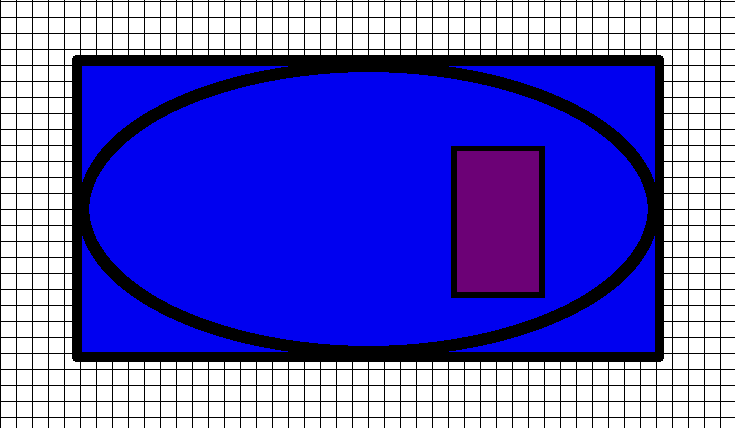
\includegraphics[scale = 0.5]{Bilder/transitiveStyle.png}
\caption{Beispiel transitiver Styleinformation}
\label{transitiveStyleExample}
\end{center}
\end{figure}In \ref{transitiveStyleExample} ist zu sehen, dass die Ellipse die Farbeigenschaften des äußeren Rechtecks übernimmt, das innere Rechteck jedoch sowohl seine eigene Farbeigenschaft (rot) definiert und außerdem die Transparenz aus \textit{S2} umgesetzt ist.
Bei der Vererbung wurde bisher wie bereits erwähnt darauf geachtet, Felder der Superklassen direkt bei der Erzeugung der neuen Instanzen weiterzugeben, um rekursives Suchen der entsprechenden Attribute in Bäumen zu vermeiden. Ebenso sind hier die Prinzipien der transitiven Style-Eigenschaften über Vererbung gelöst und auch in diesem Fall wird darauf verzichtet nur Referenzen zu speichern, über die Elternknoten erreicht werden können.
Die Parserregel für ein GeometricModel beziehungsweise dessen "'Skizze"' dem \textit{GeoModel} erkennt anonyme Styles während dem Parsen. Da anonyme Styles \textbf{keine} Informationen über Elternpaare besitzen müssen, werden sie direkt instantiiert und in einem Cache hinterlegt. Der Attributsliste des entsprechenden GeoModel wird lediglich der Name des anonymen Styles mitgegeben (tatsächlich bekommt der anonyme Style intern einen generierten Namen, den der Benutzer nicht kennt). So kann weiterhin das einheitliche Medium einer Argumentenliste aus String Tupeln an die Factorys weitergegeben werden. Die entsprechende Factory löst das Argument schlussendlich über den Namen auf und erhält wieder die eigentliche Styleinstanz.
Styles werden wie andere Attribute auch in den entsprechenden Parserklassen aufgelöst und an die Konstruktoren der Modellklassen weitergegeben.
Am Beispiel des \textit{CommonLayouts} wird deutlich wie die Style Vererbung funktioniert.
Wie die anderen Parser auch, definiert das CommonLayout zuerst Variablen, welche ausgehend von geparster und geerbter Information initialisiert und später an den Konstruktor überreicht werden. Für den Styleparameter erzeugt das CommonLayout also zunächst einen neuen Style, der sich aus dem Style der Etlerninstanz und dem eigenen zusammen setzt (siehe Listing \ref{lst:generatechildstyleaufruf}).
\begin{lstlisting}[style=scala, caption = {Erzeugen eines neuen Styles über andere Styleinstanzen}, label = {lst:generatechildstyleaufruf}]
var styl:Option[Style] = Style.generateChildStyle(cache, parentStyle, geoModel.style)
\end{lstlisting}
Hier ist zu sehen wie die Styleinformationen der nächst höheren Instanz und der eigenen Style Referenz ausgewertet werden. Mehr zu der Funktion \textit{generateChildStyle} im weiteren Verlauf. Wird unter den Attributen nun beim Pattern Matching der Name eines anonymen Styles gefunden, wird dieser ebenfalls in die bestehenden Styleinformationen eingearbeitet (siehe Listing \ref{lst:caseanonymousstyle}).
\begin{lstlisting}[style=scala, caption = {Auszug aus Code Erzeugen von Kindstyles}, label = {lst:caseanonymousstyle}]
case anonymousStyle:String if cache.styleHierarchy.contains(anonymousStyle) =>
        styl = Style.generateChildStyle(cache, styl, Some(anonymousStyle))
\end{lstlisting}Was genau macht nun \textit{generateChildStyle}?
\textit{generateChildStyle} ist eine Funktion des Style Companion Objekts (siehe Listing \ref{lst:defgeneratechildstyle}).
\begin{lstlisting}[style=scala, caption = {Auszug aus Code Funktion generateChildStyle}, label = {lst:defgeneratechildstyle}]
def generateChildStyle(cache: Cache, parents:Option[Style]*):Option[Style] ={
    val parentStyles = parents.filter(_.isDefined)
    if(parentStyles.length == 1) return parentStyles.head
    else if(parentStyles.isEmpty) return None
    val childName =
        "(child_of -> "+parentStyles.map( p => p.get.name+{if(p != parentStyles.last)" & "else ""}).mkString+")"
    Some(Style(childName, Some(parentStyles.toList.map(i => i.get.name)), List[(String, String)](), cache))
}
\end{lstlisting}Die Funktion erwartet eine variable Anzahl an Styles (Scala erlaubt diese \textit{varargs} durch die Kennzeichnung *), prüft anschließend, ob es sich um gültige Argumente handelt. Im Falle, dass mehr als ein gültiges Argument unter den Eltern ist, wird ein \textbf{neuer} Style über die Factory erzeugt, der die entsprechenden Elternteile mitbekommt. Die Style Factory kümmert sich nun wieder darum, die Felder des neuen Styles anhand des \textit{latest Bound Prinzips} zu erben, wodurch ein neuer "'Kind"' Style entsteht.
Im Folgenden wird nun ein weiteres Problem adressiert.
\subsection{Modell und Skizze; Problematik der Instantiierungsreihenfolge}\label{skizze}
Über Style, Connection und Shape  ist es möglich in der Definition des allumfassenden Diagrams ebenfalls eine Style Referenz anzugeben. Effektiv soll hierdurch ein \textit{Corporate Design} realisiert werden können, welches sämtliche Eigenschaften an unterliegende Connections, Shapes und somit auch geometrische Figuren überträgt (vgl. \Myciten{gerhart:modigen_approach}{4}). Um wie bereits beschrieben die Möglichkeit zu bieten, die Modellklassen in Zukunft parallelisiert bearbeiten zu können, wurden alle Attribute der Modellklassen als \textit{vals} gekennzeichnet und sind somit Konstant. So können ruhigen Gewissens funktionale Programmierparadigmen darauf angewendet werden und entsprechender Code kann hoch parallel arbeiten. Entsprechend ist es nicht möglich eine (beispielsweise) Shape zu erzeugen, anschließend ein Diagram zu erstellen, das auf die bereits fertige Shape referenziert und ihr somit nachträglich Styleinformationen übertragen zu wollen. Die Shape ist ja bereits erstellt und alle Felder, inklusive der Styleinformationen, sind bereits aufgelöst. Hier wird nun die selbe Taktik angewandt, wie zuvor bei den geometrischen Figuren \ref{example}. Da die Erzeugung der Shape Instanzen folglich erst erfolgen darf, wenn mögliche Corporate Styleinformationen bereits gegeben sind, werden Shapes zunächst über eine Methode namens \textit{shapeSketch} geparsed. \textit{ShapeSketch} sammelt für eine angehende Shape, wie das GeoModel für angehende GeometricModels alle geparsten Informationen, löst diese aber noch \textbf{nicht} auf. Beim Einlesen eines Diagrams, werden sowohl Style als auch Shape referenziert. Erst also wenn alle nötigen Informationen vorhanden sind, wird während des Parsing Prozesses des Diagrams die Shape Skizze(\textit{ShapeSketch}) mit dem Corporate Style zu der eigentlichen Shape aufgelöst. Hierfür verfügt die ShapeSketch Klasse über eine Methode namens \textit{toShape}, die die gespeicherten Attribute an die Shape Factory übergibt. So erzeugte "'Skizzen"' sind somit nur Container um angehende Modellklassen zu einem beliebigen Zeitpunkt auflösen zu können (siehe Listing \ref{lst:shapesketch}).
\begin{lstlisting}[style=scala, caption = {Auszug aus Code Definition der ShapeSketch container Klasse}, label = {lst:shapesketch}]
case class ShapeSketch(name:String,
                       parents:Option[List[String]],
                       style:Option[Style],
                       attrs:List[(String, String)],
                       geos:List[GeoModel],
                       descr:Option[(String, String)],
                       anch:Option[String],
                       cache: Cache){
  def toShape(corporateStyle:Option[Style]) = 
      Shape(name, parents, Style.generateChildStyle(cache, corporateStyle, style),
            attrs, geos, descr, anch, cache)
}
\end{lstlisting}Außerdem wird der nun vorhandene Corporate Style und der Style der Shape, über die bereits vorgestellte Funktion \textit{Style.generateChildStyle} kombiniert. Da der Corporate Style auf diese Weise ganz oben in der Shape eingesetzt wird, verteilt er sich wie bereits beschrieben (siehe \ref{transitivestyle}) automatisch auf die unterliegenden geometrischen Formen, da die entsprechenden Factorys die überliegenden Instanzen analysiert und entsprechend erweitert. Das Problem der Erzeugungsreihenfolge zieht sich durch das gesamte Projekt. Die Abhängigkeit zu Style Instanzen lässt es nicht zu, irgendeine Modellklasse vor dem Diagram zu erzeugen, da Styleinformationen bis hin zum Diagram immer erweitert werden können.
Folglich ist es zwingend erforderlich für sämtliche Modellklassen, die von Style abhängen, Container zu erstellen, die die unaufgelösten Attribute der Modellklasse beinhalten und es ermöglichen die Erzeugung der eigentlichen Instanz auf einen späteren Zeitpunkt zu verschieben. So findet sich zu jeder Modellklasse und jeder Hilfsklasse, die von Style abhängt, eine entsprechende Containerklasse, die mit \textit{Sketch} gekennzeichnet ist:
\begin{description}
\item[Diagram] Node und NodeSketch; Edge und EdgeSketch
\item[Shape] Shape und ShapeSketch; GeometricModel und GeoModel(einzige Ausnahme, endet nicht mit Sketch)
\item[Connection] Connection und ConnectionSketch
\end{description}Diese Lösung resultiert aus der Vorgabe, dass alle Felder der Modellklassen immutabel sein sollen und dem gewählten Lösungsweg, vererbte Eigenschaften bei der Objekterzeugung zu übergeben und nicht über Referenzen auf Elternelemente beim Aufrufzeitpunkt zu suchen. Der so gewonnene Vorteil während der Benutzung der Modelle mit besseren \textit{Response Times} rechnen zu können, da die Rekursivität des Problems aufgelöst wurde, wird also im Endeffekt durch einen zusätzlichen Overhead an Speicherauslastung wieder wett gemacht. Erzeugte Container/Skizzen können nach Auflösung zur entsprechenden Instanz der Modellklasse nämlich nicht verworfen und dem \textit{Garbage Collector} überlassen werden, da weitere Diagrams ebenfalls noch in der Lage sein müssen unberührte Skizzen der Modellklassen benutzen zu können. Die Klasse \textit{SprayParser} stellt die eigentliche Schnittstelle zum Parser dar. Sie enthält alle notwendigen Methoden um das Parsen eines Strings einzuleiten. 
\begin{description}
\item[parseStyle] Zum parsen von n Styles
\item[parseShape] Zum parsen von n Shapes
\item[parseAbstractShape] Zum parsen von n abstrakten Shapes
\item[parseConnection] Zum parsen von n Connections
\item[parseAbstractConnection] Zum parsen von n abstrakten Connections in einem String
\item[parseDiagram] Zum parsen von n Diagrams in einem String
\end{description}
Diverse weitere Methoden, sind gekapselt um den SprayParser nach außen hin möglichst simpel und benutzerfreundlich zu gestalten.
Wird eine Methode mit der Kennzeichnung \textit{Abstract} zum Parsen einer Shape oder Connection benutzt, werden tatsächliche Shape bzw. Connection Instanzen zurückgeliefert, jedoch auch für diesen Prozess die entsprechenden Container Skizzen angelegt. Das dient dem Zweck, dass es für Diagrams auch möglich ist abstrakte Shapes zu referenzieren hat aber eine sehr wichtige Konsequenz. Referenziert ein Diagram eine abstrakte Shape (oder Connection), wird die entsprechende \textit{ShapeSketch} verwendet, damit corporate Styles beachtet werden können. Die bereits bestehende Shape Instanz wird im Cache sodurch aber überschrieben, da der entsprechende Container neu umgewandelt wird und der bestehende Eintrag im Cache mit dem entsprechenden \textit{Key} (Name der Shape) überschrieben wird. Abstrakte Shapes sollten also nur dann von Diagrams referenziert werden, wenn absichtlich darauf verzichtet wird, dass Unterklassen der abstrakten Shape den corporate Style des Diagrams dadurch \textbf{nicht} implizit übernehmen. Deren Styleinformationen sind ja bereits aufgelöst und können wie bereits erklärt nicht nachträglich aktualisiert werden.
Um dieses Prinzip zu verdeutlichen ein Beispiel (siehe Listing \ref{lst:beispielabstractshape}). Es wird eine Shape \textit{A} definiert, welche einen bestimmten Style benutzt und als abstrakte Shape geparst wird. Eine weitere Shape \textit{B}, die \textit{A} erweitert, wird definiert und als normale Shape geparst. Wird nun ein Diagram definiert, das umbedingt die abstrakte Shape \textit{A} referenzieren soll und ein corporate Style namens \textit{CorporateStyle} benutzt und anschließend eine neue Shape \textit{C} definiert, welche die abstrakte Shape \textit{A} erweitern soll, dann hat nun auch die Shape C die Styleinformationen von sowohl dem \textit{CorporateStyle} und dem \textit{DefaultStyle}, da die Shape, die sie referenziert von der Diagram Definition neu erzeugt worden ist.
\begin{lstlisting}[style = scala, caption = {Beispiel Aufrufe zum Provozieren einer möglicherweise ungewollten Situation durch Vererbung}, label = {lst:beispielabstractshape}]
val abstractShape = """shape A style DefaultStyle{...}"""
parser.parseAbstractShape(abstractShape)

val normalShape = """shape B extends A{...}"""
parser.parseShape(normalShape)

val diagram = """diagram D ... (style:CorporateStyle){
		node ... {
			shape:A(...)
		}
	}"""
parser.parseDiagram(diagram)

val normalShape2 = """shape C extends A{...}"""
parser.parseShape(normalShape2)
\end{lstlisting} Da abstrakte Shapes in der Regel nur erzeugt werden um gemeinsame Attribute anderer Shapes zu vereinheitlichen oder um tests mit Shapes durchzuführen, ohne ein Diagram erstellen zu müssen ist der beschriebene Fall normalerweise nicht von Belang, da Diagrams normalerweise auf keine abstrakte Shape verweisen sollten. Hier muss überlegt werden, ob sich aus dem Referenzieren von abstrakten Shapes ein zusätzlicher nützlicher Effekt ergeben kann oder ob dadurch eher eine potenzielle Fehlerquelle eingeführt wird. Je nach dem muss über eine Prüfung verhindert werden, dass Shapeinstanzen überschrieben werden können.\linebreak Wird eine Shape bzw. Connection über \textit{parseShape} bzw. \textit{parseConnection}, also ohne die Abstract Kennzeichnung, geparst werden zunächst \textbf{keine} tatsächlichen Instanzen der Modellklassen erzeugt, sondern nur die der Container Klassen \textit{ShapeSketch} bzw. \textit{ConnectionSketch}. Jetzt erscheint es an dieser Stelle paradox, dass die Methoden mit der \textit{Abstract} Kennzeichnung tatsächliche Instanzen der Modellklassen erzeugen und die ohne \textit{Abstract} Kennzeichnung nur Container Klassen. Aus Anwendersicht ergibt dies schon mehr Sinn. Als Anwender definiert man Shapes und Connections nämlich eigentlich nur dann, wenn man sie später auch in einem Diagram referenziert. Mit anderen Worten sind die tatsächlich benutzten Shapes und Connections die, die über die Methoden \textit{parseShape} bzw. \textit{parseConnection} eingelesen werden. Shapes und Connections, die man nur dafür einlesen will, um ähnliche Eigenschaften zusammenzufassen und durch Unterklassen zu diversifizieren (sinngemäß also abstrakt), werden über die Methoden \textit{parseAbstractShape} bzw. \textit{parseAbstractConnection} eingelesen.
\subsubsection{Kritik an gewählter Taktik}Im Falle, dass mit Referenzen auf Styles der Elternobjekte gearbeitet werden würde, wäre es möglich die Styleinformationen der Elterninstanz und die eigenen erst zu erzeugen, wenn sie benötigt werden. So bestünde kein Bedarf für die vorgestellten Container Klassen. Je nach dem wie tief die Vererbungshierarchie ist, würde dies jedoch beträchtliche Nachteile im Bezug auf die \textit{Responsetime} des später erzeugten graphischen Editors mit sich bringen. Die Skizzen Klassen zu den jeweiligen Modellklassen wurden in der \textit{SprayParser.scala} Datei definiert, da andere Parsingstrategien eventuell nicht mehr abhängig von ihnen sind.
\subsection{Generatorenklassen}
Die Generatorenklassen greifen auf Informationen der Modellklassen zurück um sie auf ein gewünschtes Format abbilden zu können. Jede Moellklasse hat ein entsprechendes Pendant als Generator, so hat zum Beispiel Shape einen \textit{ShapeGenerator}. Da in den Generatoren viele Informationen verarbeitet werden, sind diese wiederum in mehrere Generatorenklasen aufgeteilt. ShapeGenerator wird unter anderem durch einen \textit{GeneratorShapeDefinition} und \textit{GeneratorInspectorDefinition} unterstützt. So werden auch hier Verantwortungen logisch aufgeteilt. Prinzipiell konnten die Generatorenklassen größtenteils von der Xtext Vorlage übernommen werden. Konzeptuell wurde so nichts verändert, außer dem zugriff auf die Modellklassen und der Formatierung des auszugebenden Javascript Codes. Scala bietet zum dynamischen Erstellen von Strings Stringinterpolation zur verfügung. So kann (wie man es beispielsweise aus Shell Skripten kennt) über ein "'\textit{\$}"' Zeichen das Ausführen von Codeblöcken eingeleitet werden. Dadurch ist es möglich sogar innerhalb eines Strings dynamisch auf Kontrollstrukturen wie \textit{for Schleifen} (und prinzipiell auf die ganze Macht Scalas) zurückzugreifen.
\section{Ausführliches Beispiel}\label{example}
Nun folgt ein ausführliches Beispiel anhand einer Shapedefinition(siehe Listing \ref{lst:exampleshapedefinition}), zur Verdeutlichung der Schritte, die beim Parsen einer Modellklasse, durchlaufen werden.
\begin{lstlisting}[style=spray, caption = {Beispieldefinition für eine Shape}, label = {lst:exampleshapedefinition}]
shape EClassShape style B{
    size-min (width=4, height=6)
    rectangle {
        style (line-width=2)
        position (x=2, y=0)
        size (width=10, height=3)
        ellipse {
            position (x=0, y=36)
            size (width=30, height=30)
        }
    }
}
\end{lstlisting}Soll eine Shapedefinition wie \ref{lst:exampleshapedefinition} eingelesen und direkt in eine Shape Instanz umgewandelt werden, wird sie zunächst im SprayParser (der Standard Parserklasse) durch folgende Regeln/Parser überprüft:
\begin{lstlisting}[style=scala, caption = {Auszug aus Code Methode zum Parsen einer Shape(Sketch)}, label = {lst:defshapesketch}]
[ 1]private def shapeSketch:Parser[Shape] =
[ 2]    ("shape" ~> ident) ~
[ 3]    (("extends" ~> rep(("(?!style)".r ~> ident)<~ ",?".r))?) ~
[ 4]    (("style" ~> ident)?) ~
[ 5]    ("{" ~> rep(shapeAttribute)) ~
[ 6]    rep(geoModel) ~
[ 7]    (descriptionAttribute?) ~
[ 8]    (anchorAttribute?) <~ "}" ^^
[ 9]    {
[10]      case name ~ parent ~ style ~ attrs ~ geos ~ desc ~ anch =>
[11]      ShapeSketch(name, parent, style, attrs, geos, desc, anch, cache) 
[12]    }
\end{lstlisting}Warum die Methode/Regel in Zeile eins \textit{shapeSketch} heißt wurde in Abschnitt \ref{skizze} erklärt. Zeile zwei filtert den identifier der Shape. Zeile drei prüft auf eine optionale Angabe erweiterter Shapes. Hierbei dürfen diese nicht "`style"' heißen, da die Regel sonst verwirrt wäre, erwartet sie doch in Zeile vier eine optionale Angabe für einen benutzten Style. Zeile fünf sucht nun \textit{n} mal nach einer Regel namens shapeAttribute (siehe Listing \ref{lst:shapeattribute})
\begin{lstlisting}[style=scala, caption = {Auszug aus Code Regeln zum Parsen der Felder}, label = {lst:shapeattribute}]
private def shapeAttribute = shapeVariable ~ arguments ^^ {case v ~ a => (v, a)}
private def shapeVariable = ("""("""+Shape.validShapeVariables.map(_+"|").mkString+""")""").r ^^ {_.toString}
\end{lstlisting}\textit{validShapeVariables} ist eine Sammlung von Strings, welche die bekannten Felder einer Shape darstellt. Diese Sammlung wird zu einem regulären Ausdruck umgewandelt und unter der Regel \textit{shapeVariable} benutzt. Die Regel \textit{arguments} entstammt dem Trait \textit{CommonParserMethods}, welches jedem Parser zur Verfügung steht. So kann \textit{shapeAttribute} Tupel von Attribut \& Wert Paaren bilden. 
Shape Attribute sind lediglich primitive Datentypen und daher nicht interessant weiterzuverfolgen. In Zeile sechs von Listing \ref{lst:defshapesketch} wird ebenfalls \textit{n} mal die Regel \textit{geoModel} angewandt, welche die einzelnen Regeln einer geometrischen Figur abbildet und ein Objekt zurückliefert, das als Container(\ref{skizze}) fungiert (siehe Listing \ref{lst:defgeomodel}).
\begin{lstlisting}[style=scala, caption = {Auszug aus Code Regel zum Parsen geometrischer Figuren}, label = {lst:defgeomodel}]
private def geoModel: Parser[GeoModel] =
    geoIdentifier ~
    ((("style" ~> ident)?) <~ "{") ~
    rep(geoAttribute|anonymousStyle) ~
    (rep(geoModel) <~ "}") ^^
    {
      case name ~ style ~ attr ~ children =>
        GeoModel(name, {if(style.isDefined) Some(style.get) else None }, attr, children, [...])
    }
\end{lstlisting}Hierbei werden nicht direkt Instanzen der eigentlich gewünschten GeometricModel Klasse erzeugt, da es für die geometrischen Figuren zwingend erforderlich ist einerseits ihre entsprechende Eltern Shape Instanz zu kennen. Diese existiert zu diesem Zeitpunkt jedoch noch nicht. Außerdem müssen sie ihre Eltern GeometricModel Instanzen kennen, welche ebenfalls erst erzeugt werden können, wenn ihre Kinder existieren. Alle Felder sollen Konstanten sein und nicht nachträglich gesetzt werden. Diese Teufelsspirale wird gelöst, indem zunächst Container Objekte erstellt werden, die die Informationen speichern und umgewandelt werden, sobald ihre Abhängigkeiten geklärt sind. Sind alle Regeln überprüft und keine Fehleingaben oder fehlende Eingaben identifiziert worden, gibt es von nun an zwei Möglichkeiten weiter zu verfahren. Einer der Gründe, warum Container erstellt werden müssen wird in \ref{transitivestyle} erklärt. Wird der Container jetzt bereits der Fabrik für Shapes übergeben und somit eine fertige Shape Instanz erzeugt, können der Shape Instanz nachträglich \textbf{keine} weiteren Informationen mehr gegeben werden.
Wird die Shape bereits jetzt erzeugt, existiert sie zwar als valide Shape, ist aber nun mehr als abstrakte Shape zu betrachten, da neue Shapes sie zwar erweitern können, sie aber nicht selber in einer Diagram Instanz referenziert wird. Das Diagram würde versuchen nachträglich Styleinformationen in die Shape einzuarbeiten. Hierzu mehr in Abschnitt \ref{skizze}. Um die Bearbeitungsschritte einer Shape zu verdeutlichen reicht es hier, den Container, welcher die Information der angehenden Shape enthält, nun direkt an die Shape Fabrik (das \textit{Companion Object} der Shape Klasse) zu übergeben. Wie man in Zeile 11 sieht, wird beim Parsen einer Shape der Container ShapeSketch zurückgeliefert.
Um entweder zu Testzwecken, oder um eine abstrakte Shape zu erzeugen, kann ein String mit Shapedefinition deshalb über die Methode \textit{abstractShape} geparsed werden (siehe Listing \ref{lst:defabstractshape}).
\begin{lstlisting}[style=scala, caption = {Auszug aus Code Methode zum direkten Parsen von Shapes}, label = {lst:defabstractshape}]
private def abstractShape:Parser[Shape] = shapeSketch ^^ {case sketch => sketch.toShape(None)}
\end{lstlisting}Wie man sieht greift \textit{abstractShape} auf die Regel/Methode \textit{shapeSketch} zurück, erzeugt jedoch anschließend direkt über \textit{ShapeSketch}'s Methode \textit{toShape}, welche lediglich ein Aufruf an die \textit{Shapefactory} weiterleitet, eine valide Shape. Ab dem Aufruf \textit{toShape} übernimmt der spezialisierte Shape Parser im \textit{Companion Objekt} der Shape Klasse das Ruder und bereitet die erhaltenen Argumente so auf, dass diese an den eigentlichen Shapekonstruktor weitergegeben werden können. Dabei werden zunächst die Superklassen aufgelöst und erweitert (siehe Abschnitt \ref{sectionInheritance}). Anschließend werden über ein Pattern Matching (siehe Listing \ref{lst:attributesforeach}) die erhaltenen Attribut- und Wert Tupel aufgelöst. Beispielsweise das \textit{"'size-min"'} Attribut, das zuvor in Listing \ref{lst:exampleshapedefinition} gegeben wurde. 
\begin{lstlisting}[style=scala, caption = {Auszug aus Code Iterieren durch Attribute mit Pattern Matching}, label = {lst:attributesforeach}]
attributes.foreach{
      case ("size-min", x) =>
        val opt = parse(width_height, x).get
        if(opt.isDefined){
          size_width_min = Some(opt.get._1)
          size_height_min = Some(opt.get._2)
        }
        ...
\end{lstlisting}Auch hierbei wird an weitere Regeln delegiert (z.B. \textit{width\_height}). Herausgefilterte Werte werden vordefinierten Variablen zugewiesen, welche später an den eigentlichen Konstruktor übergeben werden. Sind so alle Attribute der Shape aufgelöst wird der private Konstruktor der Shape companion Klasse aufgerufen. Es ist darauf zu achten, dass alle Felder der erweiterbaren Modellklasse Konstanten sind (siehe Abschnitt \ref{sectionInheritance}). Dazu müssen dem Shapekonstruktor die "'Skizzen"' (die Container) der geometrischen Figuren übergeben werden. GeometricModels sollen ebenfalls immutabel sein und müssen daher bereits bei ihrer Erzeugung ihre Eltern Shape kennen. Würden die geometrischen Figuren vor der Shape Instantiierung erzeugt werden, müsste die Referenz auf die Eltern Shape nachgereicht  und die entsprechende Referenz als \textit{var} definiert werden.
Da die Erzeugung der GeometricModels im Konstruktor erfolgt, kann die umschließende Shape über \textit{this} referenziert werden. Von nun an befindet man sich im privaten Konstruktor der Shape Modellklasse. Die wohl wichtigste Aufgabe des Shape Konstruktors ist es die geometrischen Figuren zu erzeugen. Hierbei muss der Konstruktor jedoch auch beachten, dass von einer möglichen Elternshape weitere geometrische Figuren geerbt werden können (siehe Abschnitt \ref{shapeinheritance}). Deshalb werden die neu geparsten und die geerbten geometrischen Figuren zusammen in eine Liste \textit{gemerged}. Die hier benutzte Methode \textit{parseGeometricModels} (siehe Listing \ref{lst:parsegeometricmodels}), iteriert durch die Container der geometrischen Figuren und erzeugt vollwertige GeometricModels.
\begin{lstlisting}[style = scala, caption = {Auszug aus Code Methode parseGeometricModels}, label = {lst:parsegeometricmodels}]
private def parseGeometricModels
(geoModels:List[GeoModel], parentStyle:Style) =
    geoModels.foldLeft(List[GeometricModel]())((list, g) => {
    	val newGeo = g.parse(None, parentStyle)
    	if (newGeo isDefined) newGeo.get :: list else list
    	})
\end{lstlisting}In Listing \ref{lst:parsegeometricmodels} wird die \textit{parse} Methode der Container aufgerufen, welche anhand eines Matchings entscheidet um welche geometrische Figur es sich explizit handelt (z.B. Ellipse oder Rechteck etc.). Anhand dieses Matchings wird dann der spezialisierte Parser der vielen verschiedenen Klassen aufgerufen, die eine geometrische Figur beschreiben. Im Falle der obigen Beispielshape wurde ein Rechteck definiert, welches eine Ellipse beinhaltet. Ab hier geht es also in der \textit{Rectangle Fabrik} weiter (dem Companion Objekt der Rectangle Klasse). Hier werden wie in allen anderen Parsern die mitgegebenen Attribute über ein Matching aufgelöst, wobei hierfür wieder eventuell auf weitere spezialisiertere Parser zurückgegriffen wird. Zum Beispiel wird das Rectangle seine Attribute an die Parser für das \textit{CommonLayout} und die \textit{CompartmentInfo} weitergeben. Erst wenn deren Fabrikmethoden valide Ergebnisse zurück liefern wird das Rechteck erzeugt. Der private Konstruktor der Rectanlge Klasse bekommt wiederum den Container der im Beispiel beschriebenen Ellipse mit und so geht der Vorgang in der Ellipse Fabrik von vorne los. 
\section{Cache}Bisher wurde bereits einige male erwähnt, dass sich Modellklassen untereinander referenzieren. Diese Referenzierungen können aber Aufgrund der Problematik der Instantiierungsreihenfolge nicht während des Parsingvorgangs erfolgen. Sonst würde auf Objekte verwiesen werden, die selber bereits erst in der Mache sind.
Oder es geht schlicht um die Problematik, dass Styles und Shapes unabhängig voneinander definiert werden können, Shapes jedoch namentlich auf Styles verweisen. Selbst wenn es also nur darum geht Referenzen auf erstellte Styles zu behalten um sie nicht an den \textit{Garbage Collector} zu verlieren, ist ein Mechanismus nötig, der sich entsprechende Referenzen behält und wiederum bereitstellt. Da sich Diagrams, Shapes und Styles untereinander referenzieren können sollen, muss der Parser also in der Lage sein Instanzen zu erzeugen und gleichzeitig auch zu verwalten. Hierbei wurde stets darauf geachtet, dass der SprayParser keine statischen Zustände hält. Ausgehend davon, dass der Parser zukünftig in einer Multi-Client-fähigen Umgebung eingesetzt wird, ist so garantiert, dass sich verschiedene Clients niemals die selben Ressourcen teilen und somit eventuell inkonsistente Daten produzieren. Schon eine gemeinsame Abhängigkeit eines Namensraums wäre nicht wünschenswert, da Modellklassen mit gleichen Namen sonst je nach implementierung entweder Exceptions auslösen würden oder sich gegenseitig überschreiben könnten. Wenn aber keine statischen Zustände gehalten werden kann jeder Client mit einer eigenen SrpayParser Instanz kommunizieren. Außerdem kann so auf komplizierte synchronisationsmechanismen verzichtet werden. Es wird beispielsweise zunächst eine Shape geparsed, auf die ein Diagram verweisen soll. Jedoch kann das Diagram die Shape nicht referenzieren, wenn es die entsprechende Referenz gar nicht kennt. Um die Referenz auf die Shape also nicht zu verlieren, muss sie lokal gespeichert und über eine Eigenschaft erreichbar sein, welche dem Diagram (besser gesagt dem Benutzer) bekannt ist und möglichst eindeutig sein sollte. Hierfür bietet sich der Name der Shape an. Anstatt aber nun IDs in Form von Strings zu halten, sondern auf bestehende Objekte verweisen zu können, müssen die Instanzen der generierten Shapes usw. lokal in einer Map gesichert werden. Hierfür wurde eine Hilfsklasse \textit{Cache} erstellt, die Container für alle relevanten Datentypen bereitstellt. So können fertig instantiierte Objekte zwischengespeichert und bei Bedarf über die entsprechende Map der Cache Instanz referenziert werden.
\subsection{Implicits}\label{sectionimplicit}
Hier wird Gebrauch von einer sehr mächtigen Eigenschaft von Scala gemacht, den \textit{implicits}. Wenn man sich beispielsweise im Shapekonstruktor befindet und auf ein parentShape-element zugreifen will, bräuchte man normalerweise einen Aufruf wie in Listing \ref{lst:excessivecache}.
\begin{lstlisting}[style=scala, caption = {Ausführlicher Zugriff auf ein Cache Element}, label = {lst:excessivecache}]
val someShape:Shape= cache.shapeHierarchy(parent_ID).data
\end{lstlisting}Selbst Aufrufe, die wie im obigen Beispiel recht kurz ausfallen, zerstören die Lesbarkeit ohnehin schon komplexer Codezeilen. Scala erlaubt es implicits zu definieren, welche unter anderem implizite Typumwandlungen nach angegebener Methode durchführen können. Wenn in einem sogenannten \textit{package object} besagte implicits definiert werden, ist es sogar möglich das entsprechende package object in einer Quelldatei zu importieren und so die impliziten Definitionen überall in den gewünschten Scope zu bringen. Im Falle der häufig benutzten Cache Klasse, sehen Zugriffe auf den Cache nun wie in Listing \ref{lst:simplecache}.
\begin{lstlisting}[style=scala, caption = {Vereinfachter Zugriff auf ein Cache Element}, label = {lst:simplecache}]
val parentShape:Shape = parent_ID
\end{lstlisting}
\textit{parent\_ID} ist tatsächlich immernoch ein String, wird aber vom Compiler als unpassend erkannt. Daraufhin sucht er nach einer impliziten Methode, welche in der Lage ist, den String in den gewünschten Typ (hier Shape) umzuwandeln. Der Programmierer, kann seine Cache-Instanz also sogar ohne explizit auf sie zugreifen zu müssen - eben implizit - benutzen. So kann man sich auf die wesentlichen Aspekte der Problemstellung konzentrieren. In diesem Fall ist die manuelle Typisierung der \textit{parentShape} Konstante allerdings zwingend, da der Compiler sonst eine valide Zuweisung eines Strings zu einer nicht typisierten Konstante feststellen würde und daraufhin den Typ String inferieren würde. Die entsprechende Definition des implicits im package object \textit{model.parser} sieht aus wie in Listing \ref{lst:implicitdefinition}.
\begin{lstlisting}[style=scala, caption = {Auszug aus Code Definition einer Impliziten Typumwandlung}, label = {lst:implicitdefinition}]
implicit def IDtoShape(id:String)(implicit c:Cache): Shape =
c.shapeHierarchy(id).data
\end{lstlisting}Die Umwandlung der mit implicit gekennzeichneten Funktion nimmt dem Programmierer nun den Zwischenschritt ab über die Cacheinstanz die richtige Collection ausfindig zu machen und den gewünschten String aufzulösen.
Auffällig ist, dass gleich \textbf{zwei implicits} vorkommen. Ersteres kennzeichnet die Methode für den Compiler, das zweite ist ein \textit{implicit parameter}.
Da der besagte Cache pro Parserinstanz erzeugt wird um statische Bindungen prinzipiell vermeiden zu können, kann in der Methodendefinition im Grunde auf keine Cache-Instanz zugegriffen werden.
Das liegt daran, dass der Compiler ja nicht implizit weiß, in welcher Cache-Instanz er nach der ID suchen soll.
Genau das, wird dem Compiler durch das zweite implicit mitgeteilt. Man sagt ihm quasi: '\textit{Ich kennzeichne eine Cache-Instanz, nach der sollst du suchen}'.
Diese zwei einfachen Tricks, verkürzen die Verschachtelung und steigern die Lesbarkeit des Codes.
Zwar kann der Code für jemanden, der nicht weiß was implicits sind, durchaus verwirrend aussehen, der Shape variable wird immerhin eindeutig einen String zuweisen.
Doch der Code selbst, liest sich beinahe wie pseudo Code und der eigentliche Sinn erschließt sich dadurch besser.
Entgegen der \textit{dispatch} Kennzeichnung in Xtext, handelt es sich hierbei \textbf{nicht} um eine Art dynamische Erweiterung einer Klasse, sondern um eine implizite/automatisierte Typumwandlung.
Anstatt also Methoden für einen Typ zu definieren, den dieser eigentlich garnicht besitzt, nur um ein Argument in der entsprechenden Parameterliste zu sparen, bleiben die Klassen hier konsistent.
Im package object \textit{parser} sind so für alle collections, die der Cache benutzt implizite Typumwandlungen bereitgestellt.
So bleibt der Cache bis auf wenige Ausnahmen vollkommen unsichtbar für den Entwickler (wenn gewünscht).
Implicits sind zwar unwahrscheinlich mächtig, jedoch schwer wieder los zu werden (sollte dies je gewünscht werden).
Deshalb muss vorsichtig überlegt werden, ob diese Vorgehensweise der späteren Objektstruktur hilft oder sie eher undurchsichtig macht.

\chapter{Fazit}
Abschließend zu der Arbeit werden Probleme benannt, die während des Prozesses aufgekommen sind. Außerdem Wird zusammengefasst, was erreicht wurde, was evtl. versäumt wurde und welche Möglichkeiten sich in der Zukunft für das MoDiGen Projekt ergeben.
\section{Probleme}
Die Arbeit war sehr Zeitaufwendig, da die bestehende Objektstruktur, die durch die Xtext Grammatik beschrieben wurde auf Scala bezogen gelegentlich keinen oder wenig Sinn machte. Hin und wieder wurden auch Fehler in der definierten DSL entdeckt. 
Da das Umsetzen einer DSL in Scala ausgehend von einer Xtext Grammatik voraussetzt, dass entsprechende Grammatik verstanden worden ist. Dauerte es außerdem eine Weile, bis alle Unklarheiten bezüglich der Grammatik beseitigt wurden. Hin und wieder machten sich Fehler erst lange Zeit später bemerkbar, so mussten ein paar male bestehende Klassen komplett neu überarbeitet werden. Auch Xtext Sprachkenntnisse waren nötig, da z.B. die Generatoren der Xtext Sprache sonst unklar erscheinen.
Methodenaufrufe wie createColorValue, die wie in \ref{specialstyle} beschrieben worden sind,
\begin{lstlisting}[style = scala, aboveskip =0pt]
s.layout.highlighting.unallowed.createColorValue
\end{lstlisting}sind ähnlich den \textit{implicits} in Scala für Neulinge absolut unverständlich. Auch bis die Xtext Quelldateien richtig interpretiert werden konnten, verging einige Zeit.
Da das benötigte Metamodell zur Zeit der Entwicklung noch nicht einsatzbereit war, musste sich an einigen Stellen mit Mockups geholfen werden.
Da bestehende Schnittstellen, des MoDiGens nicht verletzt werden durften, musste die Objektstruktur möglichst derer entsprechen, die durch die Xtext Grammatik eingeführt wurde. Dies ist dahingehend problematisch, dass so auch unsaubere Beziehungen, wie die ColorOrGradient, oder ColorWithTransparency übernommen werden mussten.
\subsection{Scalaspezifische Probleme}
Scalaspezifische Probleme gab es tatsächlich nicht viele. Scala ist einfach zu erlernen, bietet komfortable Collections, sowie eine ausgezeichnete und einheitliche Collections API. Außerdem bietet Scala Features wie \textit{case classes} und \textit{Pattern Matching}, um nur ein paar zu nennen. Diese Features sind schnell verstanden und umsetzbar. Einzig und allein die Tatsache, dass hier ein Scala Neuling am Werk war, bremste die Arbeit erheblich aus. So wurde zunächst mit langen und sehr komplexen regulären Ausdrücken versucht, beliebige Shapedefinitionen zu parsen, was aber aufgrund der Rekursion der in sich geschachtelten geometrischen Figuren unmöglich ist. Ein Scala Kenner, hätte sofort zu den \textit{Parser Combinator} Klassen gegriffen, diese waren dem Autor zunächst aber noch nicht bekannt. Scala bietet viele Lösungen für viele Probleme, jedoch ist es insbesondere als Scala Neuling zunächst ein Labyrinth aus Möglichkeiten und oft wird erst später bemerkt, dass eine alternative Lösung besser passt. Ein tatsächlicher Nachteil von Scala gegenüber der Xtext Technik findet sich in der Implementierung der Generatorenklassen wieder. Xtext bietet für die Definition auszugebender Strings Makros an, welche es ermöglichen Kontrollstrukturen wie if-Bedingungen und Schleifen reibungslos in String Definitionen einzubringen. Scala verfügt zwar über einen ähnlich mächtiges Feature namens \textit{String Interpolation}, jedoch hat dies einen entscheidenden Nachteil: Scope. Strings wie
\begin{lstlisting}[style = scala, literate={«}{{\flqq}}1 {»}{{\frqq}}1]
"""
Stencil.groups = {
	«var i = 0»  
	«val groupSet = getNodeToPaletteMapping(diagram).keySet()»  
	«FOR group : groupSet»  
		«getVarName(group)»  : {index: «i=i+1»  , label: '«group»  ' }«IF group != groupSet.last»  ,«ENDIF»  
 	«ENDFOR»  
};
"""
\end{lstlisting}
Sind schon während sie entstehen so formatiert, wie ihr späterer Output. Das entsprechende Pendant in Scala sieht aus wie folgt:
\begin{lstlisting}[style = scala]
var i = 0
var group = ""
val groupSet = getNodeToPaletteMapping(diagram).keySet
s"""
Stencil.groups = {
	${
	for (groupName <- groupSet) yield {
		group = groupName
		getVarName(group)
	}
}: {index: ${i = i + 1}, label: '$group' }${if (group != groupSet.last) s","}
};
"""
\end{lstlisting}Scala bietet es zwar an über \textit{Escaping} \textit{\$\{\}} Codeblöcke innerhalb von Strings auszuführen, jedoch eröffnen diese Codeblöcke auch einen eigenen Scope. Zählvariablen (beispielsweise) müssen in diesem Fall im überliegenden Scope definiert werden. Da also der gesamte zusammenhängende. Dadurch ist die entstandene Formatierung nicht so gut wie die, die durch die Xtext Makros zu erreichen ist. Das ist tatsächlich nur ein kleines Ärgernis, aber der Vollständigkeit halber aufzuführen.

\section{Schlussfolgerung/Ausblick}
\subsection{Was wurde erreicht}
Die Objektstruktur wurde erfolgreich in Scala umgesetzt. Hierbei wurde darauf geachtet, dass alle Modellklassen immutabel sind. In Zukunft kann so auf funktionale Programmiertechniken zurückgegriffen werden und insbesondere paralleler Code effizient genutzt werden. Die DSLs zu Style, Shape, Connection und Diagram können erfolgreich eingelesen werden und übersetzt werden. Hierbei wurde darauf geachtet, dass eine erste Parserlogik (\textit{Lexer}) die eingelesenen Strings in einheitliche Datenformate umwandelt, sodass spezialisiertere Parser ihren Input einheitlich behandeln können. So ist der Parser relativ leicht zu erweitern. Mehrfachvererbung bei Styles war mit Scala problemlos umsetzbar. Das iterieren über Elternelemente ist mittels generischer \textit{Getter Funktionen} unwahrscheinlich einfach, im Gegensatz zu Sprachen wie Java. Auch die (Mehrfach-) Vererbung bei Shapes funktioniert wie gewünscht. Style Eigenschaften werden transitiv an unterliegende Elemente weitergegeben, wobei die hierdurch entstehenden Abhängigkeiten aus Anwendersicht statisch gebunden werden. Tatsächlich werden Style Eigenschaften natürlich dynamisch zugewiesen, der Anwender merkt hiervon jedoch nichts. Somit ist die Anwendung besonders bei großen Baumstrukturen der Modellklassen schneller, als wenn Style Eigenschaften erst bei Bedarf aufgelöst werden würden. Durch hohen Abstraktionsgrad und Features wie \textit{implicits} und \textit{apply} Methoden ist es Möglich Scala annähernd so einfach zu schreiben wie Pseudocode.
\subsection{Was wurde nicht erreicht}
Da zu Anfang entschieden wurde die Vergabe transitiver Style Eigenschaften schon bei Objekterzeugung weiterzugeben, musste später festgestellt werden, dass aufgrund der Instantiierungsreihenfolge Containerklassen notwendig sind, welche es erlauben die Erzeugung einer Modellklasse auf einen späteren Zeitpunkt zu verschieben. Dies erzeugt einen zusätzlichen Overhead an Speicherbedarf. Alle erzeugten Objekte von Modellklassen werden in einem Cache hinterlegt um es zu ermöglichen sie über ihren Namen mittels eines Mappings zu referenzieren. Auch die Skizzen, also die Containerklassen, der Modellklassen müssen in diesem Cache hinterlegt werden, um fortlaufend bei Bedarf erzeugt werden zu können. So können also die Containerklassen auch nicht nach Erzeugung einer zugehörigen Modellklasse gelöscht werden. Performanz für Speicherauslastung.
Über die Anwendung JVisualVM\cite{jvisualvm} lässt sich hierzu ein Heapdump betrachten. Beispielhaft wurden 10.000 Shapes eingelesen:
\begin{figure}[h]
	\begin{center}
		\includegraphics[width=\textwidth]{Bilder/10000shapes.png}
		\caption{Ausschnitt aus dem Heapdump, generiert durch JVisualVM}
		\label{jvisualvm}
	\end{center}
\end{figure}Ersichtlich wird, dass bei 10000 Shapes auch 10000 ShapeSketches erzeugt werden. Das ist der angesprochene zusätzliche Overhead.

\chapter*{Anhang}
Der entstandene Quellcode ist unter folgender Webadresse einzusehen:\\\url{https://github.com/muellerjHTWGKonstanz/ScalaAsGeneratorLanguage.git}

\bibliographystyle{plainnat}
\nocite{*}
\bibliography{lit}

\end{document}